\documentclass[11pt]{amsart}

\usepackage[all]{xy}
\usepackage{amsmath,amssymb,amsthm}
\usepackage{tikz}

\usetikzlibrary{decorations.pathreplacing,decorations.markings}


\usepackage{xcolor}
\def\todoit{{\color{red} $^{TODO}$}} %!!!!!!!!!!!!!!!!!!!! I CHANGED YOUR COMMAND. !!!!!!!!!!!!!!!!!!!!
%%%%%%%%%%%%%%%%%%%%%%%%%%%%%%%%%%%%%%%%%%%%%%%%%%%%%%%%%%%%%%%%%%%%%%%%%%%%%%%%%%%%%%%%%%%%%%%%%%%%%%%
%I'm trying an alternate todo note setup that will give us a quick glance at start of document of those things that need doing. The relevant package is on the next line, and the List of Todos setup is right before the \begin{document} command.
%%%%%%%%%%%%%%%%%%%%%%%%%%%%%%%%%%%%%%%%%%%%%%%%%%%%%%%%%%%%%%%%%%%%%%%%%%%%%%%%%%%%%%%%%%%%%%%%%%%%%%%
\def\ltblue{blue!20!white}
\def\ltgreen{green!20!white}

\usepackage[colorinlistoftodos, textsize=tiny]{todonotes}

%\headheight 35pt
%
%\setlength{\textwidth}{6.5in}      %%%%%%%%%%%%%%%%%%%%%%%%%%%%%%%%%%%%%%%%%%%%%%%%%%%%%%%%%%%%%%%%%%%
%\setlength{\oddsidemargin}{0in}    Is it OK if we undo these formatting commands?
%\setlength{\evensidemargin}{0in}   %%%%%%%%%%%%%%%%%%%%%%%%%%%%%%%%%%%%%%%%%%%%%%%%%%%%%%%%%%%%%%%%%%%
%\setlength{\textheight}{8.5in}
%\setlength{\topmargin}{0in}
%\setlength{\headheight}{0in}
%\setlength{\headsep}{12pt}
%\setlength{\footskip}{.5in}

\renewcommand{\theenumi}{\roman{enumi}}

\tikzset{
  % style to apply some styles to each segment of a path
  on each segment/.style={
    decorate,
    decoration={
      show path construction,
      moveto code={},
      lineto code={
        \path [#1]
        (\tikzinputsegmentfirst) -- (\tikzinputsegmentlast);
      },
      curveto code={
        \path [#1] (\tikzinputsegmentfirst)
        .. controls
        (\tikzinputsegmentsupporta) and (\tikzinputsegmentsupportb)
        ..
        (\tikzinputsegmentlast);
      },
      closepath code={
        \path [#1]
        (\tikzinputsegmentfirst) -- (\tikzinputsegmentlast);
      },
    },
  },
  % style to add an arrow in the middle of a path
  mid arrow/.style={postaction={decorate,decoration={
        markings,
        mark=at position .5 with {\arrow[#1]{stealth}}
      }}},
}


\newcommand{\oarc}[4]{
\draw[thick, postaction={on each segment={mid arrow}}] (#1,#2) ..controls (#1 + .2,#2 + .7) and (#3 - .2,#4 + .7) .. (#3,#4);
}



\def\l{{\left(}}
\def\r{{\right)}}

\def\Z{{\mathbb Z}}
\def\C{{\mathbb C}}
\def\R{{\mathbb R}}
\def\D{{\mathbb D}}
\def\H{{\mathbb H}}
\def\P{{\mathbb P}}

\def\F{{\mathcal F}}
\def\M{{\mathcal M}}
\def\O{{\mathcal O}}
\def\A{{\mathcal A}}
\def\cl{\mathcal}

\def\s{{\sigma}}
\def\t{{\tau}}
\def\k{{\kappa}}

\def\g{\gamma}
\def\a{\alpha}
\def\xibar{\bar{\xi}}

\def\Xtilde{\widetilde{X}}
\def\etilde{\tilde{e}}

\def\bs{\backslash}
\def\dot{\bullet}

\def\G{{\Gamma}}
\def\SL{\mathrm{SL}}
\def\GL{\mathrm{GL}}
\def\O{\mathrm{O}}
\def\SO{\mathrm{SO}}
\def\U{\mathrm{U}}
\def\SU{\mathrm{SU}}
\def\PSL{\mathrm{PSL}}

\def\Gtilde{\widetilde{G}}
\def\SLtilde{\widetilde{\SL}}

\def\ar{\operatorname{ar}}
\def\mr{\operatorname{mr}}
\def\fp{{\scriptstyle \bar{\bar{p}}}}
%\def\fp{f\hspace*{-3pt}_p}

\newcommand{\pp}[2][-1]{\ensuremath ^{#2}\hspace*{#1 pt}}

\def\sing{{\mathrm{sing}}}

\newcommand\id{\operatorname{id}}
\newcommand\inter{\operatorname{int}}
\newcommand\Aut{\operatorname{Aut}}
\newcommand\Gal{\operatorname{Gal}}
\newcommand\rel{\operatorname{rel}}
\newcommand\Tr{\operatorname{Tr}}
\newcommand\End{\operatorname{End}}
\newcommand\diag{\operatorname{diag}}
\newcommand\perm{\operatorname{perm}}
%\newcommand\Sp{\Sigma^{(p)}}
%\newcommand\SpPm{\Sigma^{\pm(p)}}
%\newcommand\SpM{\Sigma^{-(p)}}

\newcommand{\al}[1]{\begin{align*}#1\end{align*}}

\newtheorem{thm}{Theorem}[section]
\newtheorem{lem}[thm]{Lemma}
\newtheorem{prop}[thm]{Proposition}
\newtheorem{cor}[thm]{Corollary}
\newtheorem{conj}[thm]{Conjecture}

\theoremstyle{definition}
\newtheorem{defn}[thm]{Definition}
\newtheorem{rem}[thm]{Remark}

%\newenvironment{definition}[1][Definition]{\begin{trivlist}
%\item[\hskip \labelsep {\bfseries #1}]}{\end{trivlist}}
%\newenvironment{ex}[1][Example]{\begin{trivlist}
%\item[\hskip \labelsep {\bfseries #1}]}{\end{trivlist}}
%\newenvironment{rem}[1][Remark]{\begin{trivlist}
%\item[\hskip \labelsep {\bfseries #1}]}{\end{trivlist}}

\makeatletter
\providecommand\@dotsep{5}
\def\listtodoname{List of Todos}
\def\listoftodos{\@starttoc{tdo}\listtodoname}
\makeatother

\begin{document}

\listoftodos
%%%%%%%%%%%%%%%%%%%%%%%%%%%%%%%%%%%%%%%%%%%%%%%%%%%%%%%%%%%%%%%%%%%%%%%%%%%%%%%%%%%%%%%%%%%%%%%%%%%%%%%%%
% BLUE is for David
% GREEN is for Cornwell
%%%%%%%%%%%%%%%%%%%%%%%%%%%%%%%%%%%%%%%%%%%%%%%%%%%%%%%%%%%%%%%%%%%%%%%%%%%%%%%%%%%%%%%%%%%%%%%%%%%%%%%%%
\newpage




%\title{The Augmentation Rank of Knot Cables}
%\author{David Hemminger\footnote{The author would like to thank Dr.\ Christopher Cornwell for the advising, and everyone else for the patience.}\\ Duke University}
%\maketitle

\title{Augmentation Rank of Satellites with Braid Pattern}

\author{David R. Hemminger}
\author{Christopher R. Cornwell}

\begin{abstract}
Given a knot $K$ in $S^3$, a question raised by Cappell and Shaneson asks if the meridional rank of $K$ equals the bridge number of $K$. Using augmentations in knot contact homology we consider the persistence of equality between these two invariants under satellite operations on $K$ with a braid pattern. In particular, we answer the question in the affirmative for a large class of iterated torus knots.
\end{abstract}

\maketitle

\section{Introduction}
Let $K$ be an oriented knot in $S^3$ and denote by $\pi_K$ the fundamental group of its complement $\overline{S^3\setminus n(K)}$, with some basepoint. We call an element of $\pi_K$ a \emph{meridian} if it is represented by the oriented boundary of a disc, embedded in $S^3$, whose interior intersects $K$ positively once. The group $\pi_K$ is generated by meridians; the \emph{meridional rank} of $K$, written $\mr(K)$, is the minimal size of a generating set containing only meridians. 

Choose a height function $h:S^3\to\R$. The \emph{bridge number} of $K$, denoted $b(K)$, is the minimum of the number of local maxima of $h|_{\varphi(S^1)}$ among $\varphi:S^1\to S^3$ which realize $K$. %Equivalently, call a 2-sphere $S\subset S^3$ a bridge sphere if each ball in $S^3\setminus S$ intersects $K$ in some number $b(S,K)$ of trivial arcs. The minimum of $b(S,K)$ over all bridge spheres and all realizations of $K$ equals $b(K)$.

By considering Wirtinger's presentation of $\pi_K$ one can show that $\mr(K)\le b(K)$ for any $K\subset S^3$. Whether the bound is equality for all knots is an open question attibuted to Cappell and Shaneson \cite[Prob. 1.11]{Kir95}. Equality is known to hold for some families of knots due to work of various authors. 

Here we study \emph{augmentations} of $K$, which are maps that arise in the study of knot contact homology. To each augmentation is associated a rank, and there is a maximal rank of augmentations of a given $K$, called the \emph{augmentation rank} $\ar(K)$. For any $K$ the inequality $\ar(K)\le \mr(K)$ holds (see Section \ref{SecBG_AugRk}). We discuss the behavior of $\ar(K)$ under certain satellite operations with a braid pattern. 

To be precise, denote the group of braids on $n$ strands by $B_n$ and write $\hat{\alpha}$ for the \emph{braid closure} of $\alpha$ (see Section \ref{SecBG}, Figure \ref{fig:BClosure}). Consider $\alpha\in B_k$ and $\beta\in B_p$ and set $K = \hat{\alpha}$. Note that $\ar(K)\le k$.
%Throughout the paper only braid closures that are knots are considered.

\begin{defn} Let $\alpha_p$ be the braid in $B_{kp}$ obtained by replacing each strand of $\alpha$ by $p$ parallel copies (in the blackboard framing). Let $\gamma$ be the inclusion of $\beta$ into $B_{kp}$ by the map $\s_i\mapsto\s_i, 1\le i\le p-1$. The \emph{braid satellite} of $K$ associated to $\alpha, \beta$ is defined as $K(\alpha,\beta) = \hat{\alpha_p\gamma}$.
\label{defn:BraidSat}
\end{defn}
\todo[color=\ltgreen]{make a figure}

As defined $K(\alpha,\beta)$ depends on the choice of braid $\alpha$ that represents the companion knot $K$. To get a more intrinsic satellite construction we can require that the index $k$ of $\alpha\in B_k$ is minimal among braid closures representing $K$ (see Section \ref{SecAsSatelliteOp} for a proof of this fact). 

Note that if $\hat{\alpha}$ and $\hat{\beta}$ are each a knot, $K(\alpha,\beta)$ is also. Our principal result is the following.

\begin{thm}\label{main}
If $\alpha\in B_k$ and $\beta\in B_p$ are such that $\ar(\hat{\alpha})=k$ and $\ar(\hat{\beta})=p$, then $\ar(K(\alpha,\beta))=kp$.
\end{thm}

A corollary of Theorem \ref{main} involves Cappell and Shaneson's question for iterated torus knots. Let ${\bf p}=(p_1,\ldots,p_n)$ and ${\bf q}=(q_1,\ldots,q_n)$ be integral vectors. We write $T({\bf p},{\bf q})$ for the $({\bf p},{\bf q})$ \emph{iterated torus knot}, defined as follows. Define $T({\bf p},{\bf q})$ inductively so that, if $\hat{\bf p}, \hat{\bf q}$ are the truncated lists obtained from ${\bf p},{\bf q}$ by removing the last integer in each, then $T({\bf p},{\bf q})$ is the $(p_n,q_n)$-cable of $T(\hat{\bf p},\hat{\bf q})$. By convention $T(\emptyset,\emptyset)$ is the unknot.

The knot $T({\bf p},{\bf q})$ is well-defined when a framing convention is chosen at each stage of cabling. In contrast to the traditional choice of Seifert framing at each stage, we choose a framing so that if $\alpha$ is of minimal braid index such that $T(\hat{\bf p},\hat{\bf q}) = \hat{B}$ then $T({\bf p},{\bf q}) = K(\alpha,(\s_1\ldots\s_{p_n-1})^{q_n})$.

\begin{cor}\label{cor:iteratedCables}
Given integral vectors ${\bf p}$ and ${\bf q}$, suppose that $|p_i|<|q_i|$ and $\text{gcd}(p_i,q_i)=1$ for each $1\le i\le n$. Then $\ar(T({\bf p},{\bf q}))=p_1p_2\ldots p_n$. Moreover, $\mr(T({\bf p},{\bf q})) = b(T({\bf p},{\bf q}))$ for all such ${\bf p}$ and ${\bf q}$.
\end{cor}

Our assumption that $|p_i|<|q_i|$ in Corollary \ref{cor:iteratedCables} is needed for the hypothesis of Theorem \ref{main} that the braids associated to the satellite have closures with augmentation rank equal to the braid index. In fact, this is not only a deficiency of our techniques; there are families of cables of $(n,n+1)$ torus knots which do not attain the large augmentation rank in Corollary \ref{cor:iteratedCables}.

\begin{thm}\label{ThmNNPlus1}For $p>1$ and $n>1$, let $K=T((n,p),(n+1,1))$. Then $\ar(K) < pn$.
\end{thm}
%\begin{rem} Using the more standard cable notation, $K$ is the $(p,p(n-1)(n+1)+1)$-cable of the $(n,n+1)$ torus knot.\end{rem}

It is natural to wonder if the augmentation rank is multiplicative under assumptions on $\alpha, \beta$ weaker than those in Theorem \ref{main}. The following is a possible generalization.

\begin{conj}Suppose $K=\hat{\alpha}$ for $\alpha\in B_k$, and that $\alpha$ has minimal index among braids with the same closure. Let $\beta\in B_p$. Then $\ar(K(\alpha,\beta)) \ge \ar(\hat{\alpha})\ar(\hat{\beta})$.
\label{ConjSuperMultipl}
\end{conj}

\begin{rem}There are examples when the inequality of Conjecture \ref{ConjSuperMultipl} is strict (see Section \ref{SecComments}).
\label{RemStrictlySuper}
\end{rem}

%Let $\tau_{m,l} \in B_{pk}$ be defined by $\tau_{m,l} = \s_m\s_{m+1}\cdots\s_{m+l-1}$, and let $\Sp_n\in B_{pk}$ be defined by $\Sp_n = \tau_{np,p}\tau_{np-1,p}\cdots\tau_{np-p+1,p}$ (see Figure \ref{FigSigma2}). Then if $\alpha\in B_k$ is given by the braid word $\s_{n_1}\s_{n_2}\cdots\s_{n_m}$, we define the \emph{$p$-copy} $\fp B$ of $B$ to be $\fp B = \Sp_{n_1}\Sp_{n_2}\cdots\Sp_{n_m}$. Our main result shows that certain satellites with a braid pattern of knots with augmentation rank equal to braid index also have augmentation rank equal to bridge index.

%FigSigma2
%\begin{figure}[ht]
%\begin{tikzpicture}[xscale=0.5,yscale=0.4,>=stealth]
%\draw(0,2)--(4,4);
%\draw(0,3)--(4,5);
%\draw[very thick,draw=white,double=black](0,4)--(4,2);
%\draw[very thick,draw=white,double=black](0,5)--(4,3);
%\draw(0,0)--(4,0);
%\draw(0,1)--(4,1);
%\draw(2.5,-1) node {$\Sigma_1$};
%\end{tikzpicture}
%\caption{$\Sigma^{(2)}_1$}
%\label{FigSigma2}
%\end{figure}


The paper is organized as follows. In Section \ref{SecBG} we give the needed background in knot contact homology, specifically Ng's cord algebra, and discuss augmentation rank and the relationship to meridional rank. Section \ref{SecBG_AugExist} has a review of techniques to be used in the proof of Theorem \ref{main}. Section \ref{SecMain} is devoted to the proof of Theorem \ref{main}, its requisite supporting lemmas, and Corollary \ref{cor:iteratedCables}. Finally, Section \ref{SecComments} considers the sharpness of our results. We prove Theorem \ref{ThmNNPlus1} and briefly discuss the more general case and Conjecture \ref{ConjSuperMultipl}.



%\begin{cor}\label{cor:cables}
%Let $K$ be a knot with augmentation rank equal to its braid index, and let $p,q>0$ with $\gcd(p,q) = 1$ and $p<q$. Then the $(p,q)$-cable of $K$ taken with the blackboard framing has augmentation rank equal to its braid index.
%\end{cor}




%\newtheorem*{thm:RanknAugs}{Theorem \ref{thm:RanknAugs}}
%  \begin{thm:RanknAugs}[\cite{Cor13a}] If $K$ is the closure of $B\in B_n$ and has a rank $n$ augmentation $\epsilon:\A_n\otimes R_0\to\C$, then 
%    \begin{equation*}\tag{\ref{eqn:FindingAugs}}
%    \epsilon(\Phi_B^L)=\Delta(B)=\epsilon(\Phi_B^R).
%    \end{equation*}
%    Furthermore, any homomorphism $\epsilon:\A_n\to\C$ which satisfies (\ref{eqn:FindingAugs}) can be extended to $\A_n\otimes R_0$ to produce a rank $n$ augmentation of $K$. 
%  \end{thm:RanknAugs}






%Define ar
%generated by entries of $A_{ij}$


\section{Satellite operators and the braid satellite}
\label{SecAsSatelliteOp}

Definition \ref{defn:BraidSat} of the braid satellite $K(\alpha,\beta)$ produces a satellite of $\hat{\alpha}$. As defined, the resulting satellite depends on the chosen braid representative of $\hat{\alpha}$. We remark here how to avoid this ambiguity.

A tubular neighborhood of a null-homologous knot $K$ in a 3-manifold has a standard identification with $S^1\times D^2$ determined by an oriented Seifert surface that it bounds. As per the usual convention, given a knot $P\subset S^1\times D^2$, let $P(K)$ denote the satellite obtained with this framing.

\begin{prop}\label{PropAsSatelliteOp}Given a knot $K$ and a braid $\beta\in B_p$, let $\omega$ be the writhe of a minimal index closed braid representing $K$. Let $P\subset S^1\times D^2$ be the braid closure of $\Delta^{2\omega}\beta$, where $\Delta^2$ is the full twist in $B_p$. Then $K(\alpha,\beta) = P(K)$ for any minimal index braid $\alpha$ with $K=\hat{\alpha}$.
\end{prop}
\begin{proof}The principal observation is that, since the Jones conjecture holds \cite{DP12,LM12}, the writhe of $\alpha$ must be $\omega$. Thus the blackboard framing of the closure of $\alpha_p\Delta^{-2\omega}$ agrees with the $(p,0)$-cable of $K$ (with Seifert framing).
\end{proof}

As a consequence, the satellite $T({\bf p},{\bf q})$ corresponds to the $(p_n,p_n\omega_n+q_n)$-cable of $T(\hat{\bf p},\hat{\bf q})$, where $\omega_n$ is defined inductively by $\omega_n=p_{n-1}\omega_{n-1}+(p_{n-1}-1)q_{n-1}$, with $\omega_1=0$.

\section{Background}
\label{SecBG}

  We review in Section \ref{SecBG_KCHdef} the construction of $HC_0(K)$ from the viewpoint of the combinatorial knot DGA, which was first defined in \cite{Ng08}; our conventions are those given in \cite{Ng12}. In Section \ref{SecBG_AugRk} we discuss augmentations in knot contact homology and their rank, which gives a lower bound on the meridional rank of the knot group. Section \ref{SecBG_AugExist} contains a discussion of techniques from \cite{Cor13a} that we use to calculate the augmentation rank.

  Throughout the paper we denote by $B_n$ the group of $n$-braids. We orient $n$-braids from left to right, labeling the strands $1,\ldots, n$, with 1 the topmost and $n$ the bottommost strand. We work with Artin's generators $\{\sigma_i^{\pm}$, $i=1,\ldots,n-1\}$ of $B_n$, where in $\s_i$ only the $i$ and $i+1$ strands interact, and they cross once in the manner depicted in Figure \ref{fig:BraidGens}.
      \begin{figure}[ht]
        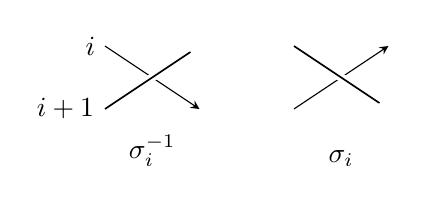
\begin{tikzpicture}[scale=0.4,>=stealth]
        \draw[->] (0,2) -- node[at start,left]{$i$} (3,0);
        \draw[draw=white,very thick,double=black,->] (0,0) -- node[at start,left]{$i+1$} (3,2);
        \draw (1.5,-0.5) node[below] {$\sigma_i^{-1}$};

        \draw[->] (6,0) -- (9,2);
        \draw[draw=white,very thick,double=black,->] (6,2) -- (9,0);
        \draw (7.5,-1) node[below] {$\sigma_i$};
        \end{tikzpicture}
        \caption{Generators of $B_n$}
        \label{fig:BraidGens}
      \end{figure}
    Given a braid $\alpha$ the braid closure $\hat{\alpha}$ of $\alpha$ is the link obtained as shown in Figure \ref{fig:BClosure}. The \emph{writhe} (or algebraic length) of $\alpha$, denoted $\omega(\alpha)$, is the sum of exponents of the Artin generators in a word representing $\alpha$.

    \begin{figure}[ht]
      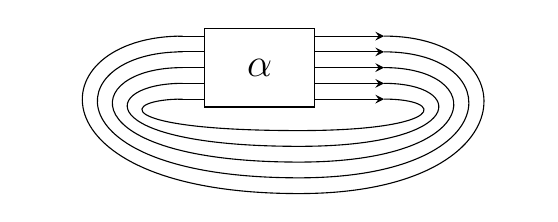
\begin{tikzpicture}[scale=0.4,>=stealth]
      %  \clip (-.7,-1.25) rectangle (7.3,2.5);
        \draw(0,-.25)--(0,2.25)--(3.5,2.25)--(3.5,-.25)--cycle;
        \draw(1.75,1) node {{\Large $\alpha$}};
        \foreach \y in {0,.5,1,1.5,2}
      %    \filldraw (4.75,\y) circle (2pt);
        \foreach \y in {0,.5,1,1.5,2}
          \draw(-.85,\y) -- (0,\y);
        \foreach \y in {0,.5,1,1.5,2} 
          \draw[thin] (3.5,\y) -- (5.25,\y);
        \foreach \y in {0,.5,1,1.5,2} 
          \draw[->] (5.18,\y) -- (5.7,\y);
        \foreach \y in {0,.5,1,1.5,2}
          \draw (5.7,\y) ..controls (7.7+\y*1.3,\y) and (7.7+\y*1.3,-\y-1) ..(3,-\y-1)
                  ..controls (-3-\y*1.3,-\y-1) and (-2.7-\y*1.3,\y)..(-.7,\y);
      %  \draw[red,->]
      %      (4.75,.5) ..controls (5.05,.75) and (5.05,1.25) ..(4.75,1.5);
      %  \draw[draw=white,double=black,very thick]
      %      (4.45,2.1)  ..controls (4.5,2.35) and (4.6,2.5) .. (4.8,2.5)
      %            ..controls (5,2.5) and (5.2,2) .. (5.2 ,1)
      %            ..controls (5.2,0) and (5,-.5) .. (4.8,-.5)
      %            ..controls (4.6,-.5) and (4.5,-.35)..(4.45,-.1);
      %  \draw   (4,-.6) node {{\footnotesize $D$}};
      %  \draw (6.15,1.95) node {{\large $\ast$}};
      %  \draw (-.65,.5) node {{\footnotesize $i$}}
      %      (-.65,1.5) node{{\footnotesize $j$}};
      \end{tikzpicture}
      \caption{The braid closure of $\alpha$}
      \label{fig:BClosure}
    \end{figure}

\subsection{Knot contact homology}
\label{SecBG_KCHdef}

  We review the construction of the combinatorial knot DGA of Ng (in fact, we discuss only the degree zero part as this will suffice for our purposes). This DGA was defined in order to be a calculation of knot contact homology and was shown to be so in \cite{EENS12} (see \cite{Ng12} for more details). Let $\A_n$ be the noncommutative unital algebra over $\Z$ freely generated by $a_{ij}$, $1\le i\ne j\le n$. We define a homomorphism $\phi : B_n \rightarrow\Aut \A_n$ by defining it on the generators of $B_n$:

  \begin{equation}
  \phi_{\s_k}\colon
  \left\{
       \begin{array}{lr}
         a_{ij}\mapsto a_{ij} & i,j\ne k,k+1\\
         a_{k+1,i}\mapsto a_{ki} & i\ne k,k+1\\
         a_{i,k+1}\mapsto a_{ik} & i\ne k,k+1\\
         a_{k,k+1}\mapsto -a_{k+1,k} & \\
         a_{k+1,k}\mapsto -a_{k,k+1} & \\
         a_{ki}\mapsto a_{k+1,i} - a_{k+1,k}a_{ki} & i\ne k,k+1\\
         a_{ik}\mapsto a_{i,k+1} - a_{ik}a_{k,k+1} & i\ne k,k+1\\
       \end{array}
  \right.
  \label{DefnPhiMap}
  \end{equation}

  Let $\iota\colon B_n \rightarrow B_{n+1}$ be the inclusion $\s_i\mapsto\s_i$ so that the $(n+1)$ strand does not interact with those from $\alpha\in B_n$, and define $\phi_\alpha^*\in \Aut \A_{n+1}$ by $\phi_\alpha^* = \phi_\alpha\circ\iota$. We then define the $n\times n$ matrices $\Phi_\alpha^L$ and $\Phi_\alpha^R$ with entries in $\A_n$ by

  $$\phi_\alpha^*(a_{i,n+1}) = \sum_{j=1}^n(\Phi_\alpha^L)_{ij}a_{j,n+1}$$

  $$\phi_\alpha^*(a_{n+1,i}) = \sum_{j=1}^na_{n+1,j}(\Phi_\alpha^R)_{ji}$$

  Finally, let $R_0$ be the Laurent polynomial ring $\Z[\lambda^{\pm1},\mu^{\pm1}]$ and define matrices $\bf{A}$ and $\bf{\Lambda}$ over $R_0$ by

  \begin{equation}
  {\bf A}_{ij} = 
  \left\{
       \begin{array}{lr}
        a_{ij} & i<j\\
        -\mu a_{ij} & i>j\\
        1-\mu & i = j\\
       \end{array}
  \right.
  \label{def:Amatrix}
  \end{equation}
  \begin{equation}
  {\bf \Lambda} = \diag[\lambda\mu^{\omega(\alpha)},1,\ldots,1].
  \label{defn:Lambda}
  \end{equation}

  \begin{defn}
  Suppose that $K$ is the closure of $\alpha\in B_n$. Define $\mathcal{I}\subset \A_n\otimes R_0$ to be the ideal generated by the entries of $\bf{A} - \Lambda\cdot\Phi_\alpha^L\cdot \bf{A}$ and $\bf{A} - \bf{A}\cdot\Phi_\alpha^R\cdot\Lambda^{-1}$. The \emph{degree zero homology of the combinatorial knot DGA} is $\operatorname{HC}_0(K) = (\A_n\otimes R_0)/\mathcal{I}$.
  \label{defn:HC_0}
  \end{defn}
  
  It was shown in \cite{Ng08} that the isomorphism class of $HC_0(K)$ is unchanged by the Markov moves on $\alpha$, hence $HC_0(K)$ is an invariant of the knot $K$. We only consider $HC_0(K)$ here, but there is a larger invariant, the differential graded algebra discussed in \cite{Ng12}.

  The proofs in Section \ref{SecMain} require a number of computations of $\phi_\alpha$ for particular braids $\alpha$. Such computations are greatly benefited by an alternate description of the map $\phi_\alpha$, which we now give and will use without comment in Section \ref{SecMain}.

  Let $D$ be a flat disk, to the right of $\alpha$, with $n$ points (punctures) where it intersects $K=\hat{\alpha}$ (see Figure \ref{FigA_nGens}). We assume the $n$ punctures of $D$ to be collinear, on a line that separates $D$ into upper and lower half-disks. Denote by $c_{ij}$ the isotopy class (fixing endpoints) of a path that is contained in the upper half-disk of $D$, with initial endpoint on the $i^{th}$ strand and terminal endpoint on the $j^{th}$ strand.

  \begin{figure}[ht]
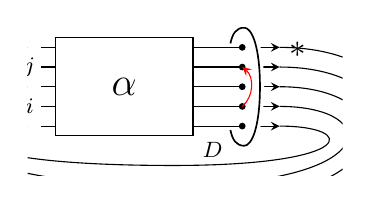
\begin{tikzpicture}[scale=0.5,>=stealth]
  \clip (-.7,-1.25) rectangle (7.3,2.5);
  \draw(0,-.25)--(0,2.25)--(3.5,2.25)--(3.5,-.25)--cycle;
  \draw(1.75,1) node {{\Large $\alpha$}};
  \foreach \y in {0,.5,1,1.5,2}
    \filldraw (4.75,\y) circle (2pt);
  \foreach \y in {0,.5,1,1.5,2}
    \draw(-.35,\y) -- (0,\y);
  \foreach \y in {0,.5,1,1.5,2} 
    \draw[thin] (3.5,\y) -- (4.75,\y);
  \foreach \y in {0,.5,1,1.5,2} 
    \draw[->] (5.18,\y) -- (5.7,\y);
  \foreach \y in {0,.5,1,1.5,2}
    \draw (5.7,\y) ..controls (7.7+\y*1.3,\y) and (7.7+\y*1.3,-\y-1) ..(3,-\y-1)
            ..controls (-3-\y*1.3,-\y-1) and (-2.7-\y*1.3,\y)..(-.7,\y);
  \draw[red,->]
      (4.75,.5) ..controls (5.05,.75) and (5.05,1.25) ..(4.75,1.5);
  \draw[draw=white,double=black,very thick]
      (4.45,2.1)  ..controls (4.5,2.35) and (4.6,2.5) .. (4.8,2.5)
            ..controls (5,2.5) and (5.2,2) .. (5.2 ,1)
            ..controls (5.2,0) and (5,-.5) .. (4.8,-.5)
            ..controls (4.6,-.5) and (4.5,-.35)..(4.45,-.1);
  \draw   (4,-.6) node {{\footnotesize $D$}};
  \draw (6.15,1.95) node {{\large $\ast$}};
  \draw (-.65,.5) node {{\footnotesize $i$}}
      (-.65,1.5) node{{\footnotesize $j$}};
\end{tikzpicture}
\caption{Cord $c_{ij}$ of $K=\hat \alpha$}
\label{FigA_nGens}
\end{figure}

  Consider $\alpha$ as a mapping class and let $\alpha\cdot c_{ij}$ denote the isotopy class of the path to which $c_{ij}$ is sent. If $D$, as viewed from the left (as pictured), is oriented as the plane then $\s_k$ acts by rotating the $k\textrm{-}$ and $(k+1)\textrm{-}$punctures an angle of $\pi$ about their midpoint in counter-clockwise fashion. Consider the \emph{algebra of paths} over $\Z$ generated by isotopy classes of paths in $D$ with endpoints on punctures, modulo the relation in Figure \ref{FigRelnPathAlg} (paths depicted there are understood to agree outside the neighborhood of the puncture shown). It was shown in \cite{Ng05} that the algebra map to $\cl A_n$ defined by $F(c_{ij})=a_{ij}$ if $i<j$, and $F(c_{ij})=-a_{ij}$ if $i>j$ satisfies $F(\alpha\cdot c_{ij}) = \phi_B(F(c_{ij}))$.

  \begin{figure}[ht]
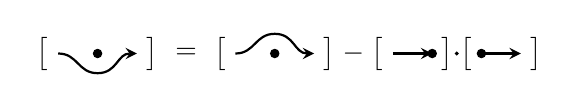
\begin{tikzpicture}[scale=0.5,>=stealth]
  \filldraw (-1,1) circle (3pt)
        (3.5,1) circle (3pt)
        (7.5,1) circle (3pt)
        (8.75,1)circle(3pt);
  \filldraw   (8.125,1) circle(1pt);
  \draw[thick,->] 
        (-2,1) ..controls (-1.5,1) and (-1.5,.5) ..(-1,.5)
             ..controls (-.5,.5) and (-.5,1) ..(0,1);
  \draw[thick,->] 
        (2.5,1) ..controls (3,1) and (3,1.5) ..(3.5,1.5)
             ..controls (4,1.5) and (4,1) ..(4.5,1);
  \draw[thick,->] (6.5,1) -- (7.5,1);
  \draw[thick,->] (8.75,1) -- (9.75,1);
  %symbols
  \draw (1.25,1) node {$=$}
      (5.5,1) node {$-$};
  \foreach \x in {-2,2.5,6.5,8.75}
  \draw (\x,1) node[left] {$\big[$};
  \foreach \x in {0,4.5,7.5,9.75}
  \draw   (\x,1) node[right] {$\big]$};     
\end{tikzpicture}
\caption{Relation in the algebra of paths}
\label{FigRelnPathAlg}
\end{figure}
  
  Let $\text{perm}:B_n\to S_n$ denote the homomorphism from $B_n$ to the symmetric group sending $\s_k$ to the simple transposition interchanging $k, k+1$. We will make use of the following.

  \begin{lem} For some $\alpha\in B_n$ and $1\le i\ne j\le n$, consider $(\Phi_\alpha^L)_{ij}\in \A_n$ as a polynomial expression in the (non-commuting) variables $\{a_{kl}, 1\le k\ne l\le n\}$. Writing $i'=\text{perm}(\alpha)(i)$, every monomial in $(\Phi_\alpha^L)_{ij}$ is a constant times $a_{i'i_1}a_{i_1i_2}\ldots a_{i_{l-1},j}$ for some $l\ge 0$, the monomial being a constant if $l=0$ and only if $i'=j$.
  \label{lem:monomial}
  \end{lem}
  \begin{proof}Include $\alpha$ in $B_{n+1}$ and consider the isotopy class of the path $\alpha\cdot c_{i,n+1}$ which begins at $i'$ and ends at $n+1$ (as $\alpha$ does not interact with the $(n+1)$ strand. Applying the relation in Figure \ref{FigRelnPathAlg} to the path equates it with a sum (or difference) of another path with the same endpoints and a product of two paths, the first beginning at $i'$ and the other ending at $n+1$. A finite number of applications of this relation allows one to express the path as a polynomial in the $c_{kl}, 1\le k\ne l\le n$ where each monomial has the form $c_{i'i_1}\ldots c_{i_{l-1},j}$. The result then follows from the fact that $\phi_\alpha(a_{i,n+1}) = \phi_\alpha(F(c_{i,n+1})) = F(\alpha\cdot c_{i,n+1})$.

  Alternatively, the statement follows from noting that (\ref{DefnPhiMap}) defining $\phi_{\s_k}$ has the desired property and that $\phi:B_n\to\text{Aut}(\A_n)$ is a homomorphism.
  \end{proof}

\subsection{Augmentations and augmentation rank}
\label{SecBG_AugRk}

  Let $S$ be a ring with 1, and consider it a differential graded algebra supported in grading 0, with trivial differential. Augmentations of $(\A,\partial)$ are DGA maps $(\A,\partial)\to (S,0)$. For our setting, if $\alpha\in B_n$ is a braid representative of $K$, such a map corresponds precisely to a homomorphism $\epsilon:\A_n\otimes R_0\to\C$ such that $\epsilon$ sends each generator of $\mathcal I$ to zero (see Definition \ref{defn:HC_0}).

  \begin{defn}
  Suppose that $K$ is the closure of $\alpha\in B_n$. An \emph{augmentation} of $K$ is a homomorphism $\epsilon: \A_n\otimes R_0\rightarrow \C$ such that each element of $\mathcal I$ is sent by $\epsilon$ to zero.
  \label{defn:Aug}
  \end{defn}

  A correspondence between augmentations and particular representations of the knot group $\pi_K$ were studied in \cite{Cor13a}. Recall that $\pi_K$ is generated by meridians. We may fix a meridian $m$ and generate $\pi_K$ by conjugates of $m$.

  \begin{defn}
  For any integer $r\ge1$, a homomorphism $\rho:\pi_K\to\text{GL}_r\C$ is a \emph{KCH representation} if there is a meridian $m$ of $K$ such that $\rho(m)$ is diagonalizable and has an eigenvalue of 1 with multiplicity $r-1$. We call $\rho$ a \emph{KCH irrep} if it is irreducible.
  \label{defn:KCHReps}
  \end{defn}

  In \cite{Ng08}, Ng describes an isomorphism between $HC_0(K)$ and an algebra constructed from elements of $\pi_K$. As discussed in \cite{Ng12} a KCH representation $\rho:\pi_K\to\text{GL}_r\C$ induces an augmentation $\epsilon_\rho$ of $K$. Given an augementation, the first author showed how to construct a KCH representation that induces it. In fact, we have the following rephrasing of results from \cite{Cor13a}.

  \begin{thm}[\cite{Cor13a}]
  Let $\epsilon:\A_n\otimes R_0\to\C$ be an augmentation with $\epsilon(\mu)\ne 1$. There is a KCH irrep $\rho:\pi_K\to\text{GL}_r\C$ such that $\epsilon_\rho=\epsilon$. Furthermore, for any KCH irrep $\rho:\pi_K\to\text{GL}_r\C$ such that $\epsilon_\rho = \epsilon$, $r$ equals the rank of $\epsilon({\bf A})$.
  \label{thm:AugKCH_Corresp}
  \end{thm}

  Considering Theorem \ref{thm:AugKCH_Corresp} we make the following definition.

  \begin{defn}
  The \emph{rank} of an augmentation $\epsilon:\A_n\otimes R_0\to\C$ with $\epsilon(\mu)\ne 1$ is the rank of $\epsilon({\bf A})$. Given a knot $K$, the \emph{augmentation rank of} $K$, denoted $\text{ar}(K)$, is the maximum rank among augmentations of $K$.
  \label{defn:AugRk}
  \end{defn}

  \begin{rem} The augmentation rank can be defined for target rings other than $\C$, but this paper only considers augmentations as in Definition \ref{defn:Aug}.
  \end{rem}

  It is the case that $\text{ar}(K)$ is well-defined. That is, given $K$ there is a bound on the maximal rank of an augmentation of $K$.

  \begin{thm}[\cite{Cor13b}] Given a knot $K\subset S^3$, if $g_1,\ldots,g_d$ are meridians that generate $\pi_K$ and $\rho:\pi_K\to\text{GL}_r\C$ is a KCH irrep then $r\le d$.
  \label{thm:DimBound}
  \end{thm}

  As in the introduction, if we denote the meridional rank of $\pi_K$ by $\text{mr}(K)$, then Theorem \ref{thm:DimBound} implies that $\text{ar}(K)\le\text{mr}(K)$. In addition, the geometric quantity $b(K)$ called the bridge index of $K$ is never less than $\text{mr}(K)$. Thus we have the following corollary.
    
\begin{cor}[\cite{Cor13b}] Given a knot $K\subset S^3$,
$$\text{ar}(K)\le\text{mr}(K)\le b(K)$$
\label{cor:DimBound}
\end{cor}

  As a result, to verify for $K$ that $\text{mr}(K)=b(K)$ it suffices to find an augmentation of $K$ with rank equal to $b(K)$. As we discuss in the next section, we will concern ourselves in this paper with a setting where $\text{ar}(K)=n$ and there is a braid $\alpha\in B_n$ which closes to $K$. This is a special situation, since $b(K)$ is strictly less than the braid index for many knots.

\subsection{Finding augmentations}
\label{SecBG_AugExist}
  The following theorem concerns the behavior of the matrices $\Phi_\alpha^L$ and $\Phi_\alpha^R$ under the product in $B_n$. It is an essential tool for studying $HC_0(K)$ and will be central to our arguments.

  \begin{thm}[\cite{Ng05}, Chain Rule] Let $\alpha,\gamma$ be braids in $B_n$. Then $\Phi_{\alpha\gamma}^L = \phi_\alpha(\Phi_{\gamma}^L)\cdot\Phi_\alpha^L$ and $\Phi_{\alpha\gamma}^R = \Phi_\alpha^R\cdot\phi_\alpha(\Phi_{\gamma}^R)$.
  \label{thm:ChainRule}
  \end{thm}
  %%possibly CHANGE THE NAMES of \alpha and \gamma here

  The main result of this paper concerns augmentations with rank equal to the braid index of the knot $K$. Define the diagonal matrix $\Delta(\alpha)=\text{diag}[(-1)^{w(\alpha)},1,\ldots,1]$. The following statement follows from results in \cite[Section 5]{Cor13b}.\todo{but the theorem is marked Cor13a?}

  \begin{thm}[\cite{Cor13a}] If $K$ is the closure of $\alpha\in B_n$ and has a rank $n$ augmentation $\epsilon:\A_n\otimes R_0\to\C$, then 
    \begin{equation}
    \epsilon(\Phi_\alpha^L)=\Delta(\alpha)=\epsilon(\Phi_\alpha^R).
    \label{eqn:FindingAugs}
    \end{equation}
    Furthermore, any homomorphism $\epsilon:\A_n\to\C$ which satisfies (\ref{eqn:FindingAugs}) can be extended to $\A_n\otimes R_0$ to produce a rank $n$ augmentation of $K$. 
  \label{thm:RanknAugs}
  \end{thm}

  The proof of Theorem \ref{main} relies on this characterization of rank $n$ augmentations. That is, given a braid $\alpha\in B_k$ with a rank $k$ augmentation $\epsilon:\cl A_k\to\C$, and $\beta\in B_p$ with a rank $p$ augmentation $\epsilon':\cl A_p\to\C$ we show that $K(\alpha,\beta)$ has a rank $kp$ augmentation by defining a homomorphism $\psi:\cl A_{kp}\to\cl A_k\otimes\cl A_p$ so that $(\epsilon\otimes\epsilon')\circ\psi$ satisfies (\ref{eqn:FindingAugs}) for the braid $\alpha_p\gamma$.

  There is a symmetry on the matrices $\Phi_\alpha^L$ and $\Phi_\alpha^R$ that is relevant to the study of augmentations in this setting. Define an involution $x\mapsto\overline x$ on $\A_n$ (termed \emph{conjugation}) as follows: first set $\overline{a_{ij}}=a_{ji}$; then, for any $x,y\in\A_n$, define $\overline{xy}=\overline y\hspace*{1pt}\overline x$ and extend the operation linearly to $\A_n$. We have the following symmetry.

  \begin{thm}[\cite{Ng05}, Prop.\hspace*{-0.7pt} 6.2]For a matrix of elements in $\A_n$, let $\overline{M}$ be the matrix such that $\left(\overline M\right)_{ij} = \overline{M_{ij}}$. Then for $\alpha\in B_n$, $\Phi_\alpha^R$ is the transpose of $\overline{\Phi_\alpha^L}$.
  \label{thm:Transpose}
  \end{thm}

  %Define $\A_n^{ab}$ to be the quotient of $\A_n$ by the ideal generated by $\{xy-yx | x,y\in\A_n\}\cup\{a_{ij}-a_{ji} | i\ne j\}$. Any homomorphism $\epsilon:\A_n\to\C$ such that $\epsilon(a_{ij}-a_{ji})=0$ for all $i\ne j$ determines a homomorphism $\epsilon:\A_n^{ab}\to\C$. As a consequence, Theorems \ref{thm:RanknAugs} and \ref{thm:Transpose} imply that finding $\epsilon:\A_n\to\C$ such that $\epsilon(a_{ij}-a_{ji})=0$ and satisfying $\epsilon(\Phi_B^L) = \Delta(B)$ suffices to determine a rank $n$ augmentation. There do exist braids $B\in B_n$ and homomorphisms $\epsilon:\A_n\to\C$ satisfying (\ref{eqn:FindingAugs}), such that $\epsilon$ does not descend to $\A_n^{ab}$. However, to date every such braid $B\in B_n$ that has been found, also admits a homomorphism satisfying (\ref{eqn:FindingAugs}) that does descend to $\A_n^{ab}$. 

\todo[color=\ltgreen,inline]{It may be appropriate here to indicate that $\text{ar}(K)<\text{mr}(K)$ sometimes (maybe in previous subsection), and talk about the 2-cable of the trefoil that does not have $\text{ar}(K,\mathbb C)=4$}

%%%%%%%%%%%%%%%%%%%%%%%%%%%%%%%%%%%%%%%%%%%%%%%%%%%%%%%%%%%%%%%%%%%%%%%%%%%%%%%%%%%%%%%%%%%%%%%%%%%%%%%%%%%%%%%%%%%%%%%%%%%%%%%%%%%%%%%%%%%%
%%%%%%%%%%%%%%%%%%%%%%%%%%%%%%%%%%%%%%%%%%%%%%%%%%%%%%%%%%%%%%%%%%%%%%%%%%%%%%%%%%%%%%%%%%%%%%%%%%%%%%%%%%%%%%%%%%%%%%%%%%%%%%%%%%%%%%%%%%%%

\section{Main Result}
\label{SecMain}
\todo[color=\ltblue,inline]{figure out this two tensor products nonsense}

\todo[inline]{how do I bring in equations to fit margins?}

We begin in Section \ref{MainProof} with our main theorem. The proof relies upon an intermediate result, Proposition \ref{psiofbp}, which is shown in the subsequent Section \ref{PropAndLemmas} along with some supporting lemmas. 

\subsection{Proof of main result}
\label{MainProof}
In this section we prove our main result, which we now recall. The notation of Theorem \ref{main} will be used throughout Section \ref{SecMain}.

\newtheorem*{main}{Theorem \ref{main}}
\begin{main}
If $\alpha\in B_k$ and $\beta\in B_p$ are such that $\ar(\hat{\alpha})=k$ and $\ar(\hat{\beta})=p$, then $\ar(K(\alpha,\beta))=kp$.
\end{main}

Theorem \ref{main} is proved by defining an algebra map $\psi\colon \A_{pk} \rightarrow \A_k\otimes \A_p$ such that $\psi(\Phi_{\alpha\gamma}^L)$ factors suitably across the tensor product. This is the content of Proposition \ref{psiofbp}, which follows from Lemmas \ref{commutes} and \ref{basecase}, the former following from a calculation (Lemma \ref{Sigma_n}) and the latter depending on the former. 

%We begin with the definition of $\psi$ and statement of Proposition \ref{psiofbp}, followed by the proof of Proposition \ref{psiofbp} and Lemmas \ref{commutes}, \ref{basecase}, and \ref{Sigma_n}.

%As we saw in the introduction, Theorem \ref{main} has an immediate corollary, which follows from Corollary \ref{cor:DimBound} and Theorem 1.3 from \cite{Cor13b}:

%\newtheorem*{cor:iteratedCables}{Corollary \ref{cor:iteratedCables}}
%\begin{cor:iteratedCables}
%Let $T$ be an iterated torus knot, and suppose it arises from taking $(p_i,q_i)$-cables such that $p_i<q_i$ for all $i$.  Then $\mr(T) = b(T)$.
%\end{cor:iteratedCables}

%To prove Theorem \ref{main}, we use a map $\psi\colon \A_{pk} \rightarrow \A_k\otimes\A_p$ with some useful properties.  An important intermediate step is Proposition \ref{psiofbp}, which we will use in conjunction with the Chain Rule to construct an augmentation $\epsilon$ from $\epsilon_k$ and $\epsilon_p$.  Proposition \ref{psiofbp} will follow from Lemmas \ref{commutes} and \ref{basecase}, and Lemma \ref{basecase} depends on Lemma \ref{commutes} while Lemma \ref{commutes} depends on Lemma \ref{Sigma_n}.  We begin with the definition of $\psi$ and statement of Proposition \ref{psiofbp}, followed by the proof of Proposition \ref{psiofbp} and Lemmas \ref{commutes},\ref{basecase}, and \ref{Sigma_n}.






%Among other things, this theorem implies that iterated cables of torus knots have meridional rank equal to their bridge number.  \todo[color=\ltblue]{braid rep've info needed to make well-defined} Consider a $(r,s)$-torus knot $T$ with $\gcd(r,s) = 1$ and $r<s$. $T$ has bridge number $r$ and is the closure of a braid $B$ on $r$ strands, and since all torus knots have bridge number equal to their augmentation rank (\todo[color=\ltblue]{cite cornwell}), we have that there exists an augmentation $\epsilon_T\colon \A_r\rightarrow \C$\todo[color=\ltblue]{finish this}. .  given by the braid sum of $T^{(p)}$ with a braid who's first $p$ strands form a torus knot with bridge number (and therefore augmentation rank) equal to $p$ and such that $w(T)$ is even (i.e. a $(p,q)$ torus knot, where $\gcd(p,q) = 1$, $p<q$, and $pq-q$ is even).  Theorem \ref{main} then says that this cable has augmentation rank equal to its braid index, implying that its meridional rank is equal to its bridge number.  Furthermore, we can iterate this process, taking cables of the resulting knots with augmentation rank, bridge number, and braid index all equal.\todo[color=\ltblue]{prob from Kirby list should be mentioned here}



For each generator $a_{ij}, 1\le i\ne j\le kp$, define

\begin{equation}
\psi(a_{ij}) =
  \begin{cases}
         1\otimes a_{r_ir_j} & \colon q_i = q_j\\
         a_{q_i+1,q_j+1}\otimes 1 & \colon r_i = r_j\\
         0 & \colon (q_i-q_j)(r_i-r_j)<0\\
         a_{q_i+1,q_j+1}\otimes a_{r_ir_j} & \colon (q_i-q_j)(r_i-r_j)>0\\
  \end{cases},
  \label{defn:psi}
\end{equation}

\noindent which determines an algebra map $\psi\colon \A_{pk} \rightarrow \A_k\otimes \A_p$. Note that if $\psi(a_{ij}) \in 1\otimes \A_p$ then $q_i = q_j$ or $a_{ij}\in\ker\psi$. Also, if we extend conjugation to $\A_k\otimes\A_p$ by applying it to each factor, then $\psi(\overline{a_{ij}}) = \overline{\psi(a_{ij})}$. We have the following proposition.

\begin{prop}\label{psiofbp}
For any braid $\alpha$, $\psi\left(\Phi_{\alpha_p}^L\right) = \left(\left(\Phi_\alpha^L\right)_{ij}\otimes 1\right)\otimes I_p$ and $\psi\left(\Phi_{\alpha_p}^R\right) = \left(\left(\Phi_\alpha^R\right)_{ij}\otimes 1\right)\otimes I_p$\todo[color=\ltblue]{make consistent throughout paper}
\end{prop}


Note that here we mean the tensor product of $\Phi_\alpha^L$ and $I_p$ as matrices, not as linear maps, while the tensor product of $\left(\Phi_\alpha^L\otimes I_p\right)_{ij}$ and $1$ is a tensor product of algebra elements, so that if we divide the matrix $\psi\left(\Phi_{\alpha_p}^L\right)$ into $k^2$ $p\times p$\todo{awkward} blocks, the $ij$th block is $\left(\Phi_\alpha^L\right)_{ij}I_p$.

%It turns out that instead of $\psi$ we could have defined a simpler homomorphism $\rho\colon \A_{pk}\rightarrow \A_k$ that would take $a_{ij}$ to $a_{q_{i+1},q_{j+1}}$ if $r_i=r_j$ and 0 otherwise, and Proposition \ref{psiofbp} would still be true (this follows from the same ideas used in the proof of Proposition \ref{psiofbp}).  The advantage of $\psi$ is that it doesn't send $a_{ij}$ to 0 if $q_i=q_j$, a fact which will be important in the proof of Theorem \ref{main}.


\begin{proof}[Proof of Theorem \ref{main}]
By Theorem \ref{thm:RanknAugs} there exist augmentations $\epsilon_k\colon \A_k\otimes R_0 \rightarrow \C$ and $\epsilon_p\colon \A_p\otimes R_0 \rightarrow \C$, for the closures of $\alpha,\beta$ respectively, such that $\epsilon_k\left(\Phi_\alpha^L\right) = \epsilon_k\left(\Phi_\alpha^R\right) = \Delta(\alpha)$ and $\epsilon_p\left(\Phi_{\beta}^L\right) = \epsilon_p\left(\Phi_{\beta}^R\right) = \Delta(\beta)$. Theorem \ref{thm:RanknAugs} also implies that it suffices to prove that there exists an augmentation $\epsilon\colon \A_{pk}\otimes R_0\rightarrow \C$ such that $\epsilon\left(\Phi_{\alpha_p\gamma}^L\right) = \epsilon\left(\Phi_{\alpha_p\gamma}^R\right) = \Delta(\alpha_p\gamma)$.

Below we will define a homomorphism $\delta\colon\A_p\rightarrow \C$ such that $\delta = \pm \epsilon_p$\todo{misleading?}, the sign depending on the parity of $w(\alpha)$ and $p$. Let $\pi\colon \C\otimes \C \rightarrow \C$ be the multiplication $a\otimes b\mapsto ab$. Our desired map is defined by $\epsilon = \pi\circ(\epsilon_k\otimes\delta)\circ\psi$.

The Chain Rule theorem gives that
\begin{equation}
\pi\circ(\epsilon_k\otimes\delta)\circ\psi\left(\Phi_{\alpha_p\gamma}^L\right) = \pi\circ(\epsilon_k\otimes\delta)\psi\left(\phi_{\alpha_p}\left(\Phi_{\gamma}^L\right)\right)\psi\left(\Phi_{\alpha_p}^L\right)
\label{eqn1MainPf}
\end{equation}

Consider the homomorphism $\phi_{\alpha_p}$ through the description given in Section \ref{SecBG_KCHdef}. As each $a_{ij}, 1\le i\ne j\le p$, is represented by the isotopy class $c_{ij}$, and the leftmost $p$ punctures are moved as one block by the action of $\alpha_p$ on $D$, there is an $0\le m<k$ so that $\phi_{\alpha_p}(a_{ij})=a_{i+mp,j+mp}$ for each $i,j$ in this range. As $\psi(a_{i + mp, j+mp})=1\otimes a_{ij}$,

$$\psi\left(\phi_{\alpha_p}\left(\Phi_{\gamma}^L\right)\right) = \left(1\otimes \left(\Phi_{\beta}^L\right)_{ij}\right)$$

\noindent By Proposition \ref{psiofbp}, we have that 

$$\psi\left(\Phi_{\alpha_p}^L\right) = \left(\left(\Phi_\alpha^L\right)_{ij}\otimes 1\right)\otimes I_p = \left(\left(\Phi_\alpha^L\otimes I_p\right)_{ij}\otimes 1\right)$$\todo{this is maybe confusing, since $i,j$ in the middle part range over different values than $i,j$ on the RHS}

\noindent Returning to the right hand side of (\ref{eqn1MainPf})
\begin{align*}
\pi\circ(\epsilon_k\otimes\delta)\left(\psi\left(\phi_{\alpha_p}\left(\Phi_{\gamma}^L\right)\right)\psi\left(\Phi_{\alpha_p}^L\right)\right)
    & = \pi\circ(\epsilon_k\otimes\delta)\left(\left(1\otimes \left(\Phi_{\beta}^L\right)_{ij}\right)\left(\left(\Phi_\alpha^L\otimes I_p\right)_{ij}\otimes 1\right)\right)\\
    & = \delta\left(\Phi_{\gamma}^L\right)\left(\Delta(\alpha)\otimes I_p\right).
\end{align*}

We are done if $\delta$ may be defined so that $\delta\left(\Phi_{\gamma}^L\right)\left(\Delta(\alpha)\otimes I_p\right) = \Delta(\alpha_p\gamma)$.  When $w(\alpha)$ is even $w(\alpha_p)$ is also, and further $\Delta(\alpha)=I_k$. Letting $\delta = \epsilon_p$ makes 
\begin{equation*}
\delta\left(\Phi_{\gamma}^L\right)\left(\Delta(\alpha)\otimes I_p\right) = \epsilon_p\left(\Phi_{\gamma}^L\right) = \Delta(\gamma) = \Delta(\alpha_p\gamma).
\end{equation*}

Suppose that $w(\alpha)$ is odd. We define $g\colon \{1,\ldots,p\}\rightarrow \{\pm 1\}$ as follows. Let $x_1 = 1$, and $x_l = \perm(\gamma)(x_{l-1})$ for $1<l\le p$. Since the first $p$ strands of $\gamma$ close to a knot, $\perm(\gamma)$ is given by the $p$-cycle $(x_1x_2\ldots x_p)$. If $p$ is even, we let $g(x_1) = 1$, and $g(x_l) = -g(x_{l-1})$ for $1<l\le p$. If $p$ is odd, let $g(x_1) = g(x_2) = 1$ and $g(x_l) = -g(x_{l-1})$ for $2<l\le p$.

 Define $\delta: \A_p\to \C$ by setting $\delta(a_{ij}) = g(i)g(j)\epsilon_k(a_{ij})$ for $1\le i\ne j\le p$. Fix $i,j$ and consider a monomial $M$ in $\left(\Phi_{\gamma}^L\right)_{ij}$, which is constant if $i>p$ or $j>p$ so that $\delta(M)$ is defined. If $i,j\le p$, then writing $i'=\text{perm}(\gamma)(i)$, Proposition \ref{lem:monomial} implies $M=c_{ij}a_{i',j_1}a_{j_1,j_2}\ldots a_{j_m,j}$ for some $j_1,\ldots j_m\in \{1,\ldots,p\}$, possibly being constant only if $i'=j$, implying that 

$$\delta(M) = g(i')g(j)\left(\prod_{k=1}^m g(j_k)^2\right)\epsilon_p(M) = g(i')g(j)\epsilon_p(M).$$

\noindent Note, when $M$ is constant then $\delta(M) = M = g(i')g(j)\epsilon_p(M)$ since $i'=j$. Since this holds for each monomial, we have that

$$\delta\left(\left(\Phi_{\gamma}^L\right)_{ij}\right) = g(i')g(j)\epsilon_p\left(\left(\Phi_{\gamma}^L\right)_{ij}\right).$$

When $p$ is even, $w(\alpha_p)$ is also even and so the opposite parity of $w(\alpha)$. Our definition of $g$ gives $\delta\left(\left(\Phi_{\gamma}^L\right)_{ii}\right) = -\epsilon\left(\left(\Phi_{\gamma}^L\right)_{ii}\right)$ for $i\le p$. Thus 

$$\delta\left(\Phi_{\gamma}^L\right) = 
\left( \begin{array}{ccc}
(-1)^{w(\gamma)+1} & 0 & 0 \\
0 & -I_{p-1} & 0 \\
0 & 0 & I_{(k-1)p} \end{array} \right)
$$
\noindent and therefore
$$
\delta\left(\Phi_{\gamma}^L\right)\left(\Delta(\alpha)\otimes I_p\right) = \diag[(-1)^{w(\alpha) + w(\gamma) + 1},1\ldots 1] = \Delta(\alpha_p\gamma)
$$
\noindent as desired.

When $p$ is odd, $w(\alpha_p)$ is odd and therefore the same parity of $w(\alpha)$. Our definition of $g$ gives that $\delta\left(\left(\Phi_{\gamma}^L\right)_{11}\right) = \epsilon\left(\left(\Phi_{\gamma}^L\right)_{11}\right)$ and $\delta\left(\left(\Phi_{\gamma}^L\right)_{ii}\right) = -\epsilon\left(\left(\Phi_{\gamma}^L\right)_{ii}\right)$ for $1<i\le p$, so 

$$\delta\left(\Phi_{\gamma}^L\right) = 
\left( \begin{array}{ccc}
(-1)^{w(\gamma)} & 0 & 0 \\
0 & -I_{p-1} & 0 \\
0 & 0 & I_{(k-1)p} \end{array} \right)
$$
\noindent and therefore
$$
\delta\left(\Phi_{\gamma}^L\right)\left(\Delta(\alpha)\otimes I_p\right)= \diag[(-1)^{w(\alpha) + w(\gamma)},1\ldots 1] = \Delta(\alpha_p\gamma)
$$
\noindent as desired. 

There is little difference in the proof that $\epsilon(\Phi_{\alpha_p\gamma}^R) = \Delta(\alpha_p\gamma)$, except that monomials in $(\Phi_{\gamma}^R)_{ij}$ are of the form $c_{ij}a_{i,j_1}a_{j_1,j_2}\cdots a_{j_k,j'}$ where $j'=\text{perm}(\gamma)(j)$. Applying Theorem \ref{thm:RanknAugs} now completes the proof.
%Similarly, we have that
%$$
%\pi\circ(\epsilon_k\otimes\delta)\circ\psi\left(\Phi_{\fp B\gamma}^R\right) = \pi\circ(\epsilon_k\otimes\delta)\left(\left(\left(\Phi_B^R\otimes I_p\right)_{ij}\otimes 1\right)\left(1\otimes \left(\Phi_{\gamma}^R\right)_{ij}\right)\right)
%$$
%but since $\epsilon_k\left(\Phi_B^L\right) = \epsilon_k\left(\Phi_B^R\right)$ and $\epsilon_p\left(\Phi_{\gamma}^L\right) = \epsilon_p\left(\Phi_{\gamma}^R\right)$, in each of the above cases we have that the right hand side is equal to $\Delta\left(\fp B\gamma\right)$, which completes the proof.
\end{proof}

%\begin{align*}
%\pi\circ(\epsilon_k\otimes\delta)\left(\left(\left(\Phi_B^R\otimes I_p\right)_{ij}\otimes 1\right)\left(1\otimes \left(\Phi_{\gamma}^R\right)_{ij}\right)\right) &= \pi\circ(\epsilon_k\otimes\delta)\left(\left(\left(\Phi_B^L\otimes I_p\right)_{ij}\otimes 1\right)\left(1\otimes \left(\Phi_{\gamma}^L\right)_{ij}\right)\right)\\
%&= \Delta\left(\fp B\gamma\right)
%\end{align*}
%Which completes the proof.

\subsection{Proposition \ref{psiofbp} and supporting lemmas}
\label{PropAndLemmas}

\noindent We use the following two lemmas to prove Proposition \ref{psiofbp}.  Figure \ref{FigCommutes} demonstrates an example for Lemma \ref{commutes}, showing that $\psi(\phi_{f\hspace*{-3pt}_2\s_2}(a_{24})) = \phi_{\s_2}\otimes\id(\psi(a_{24}))$.  Note that in the figure we condense elements such as $a_{13}\otimes 1$ to $a_{13}$ and include products of algebra elements on a single set of points in order to make the notation cleaner.


\begin{lem}\label{commutes}
$\psi\circ\phi^{\pm 1}_{\fp\s_n} = \left(\phi^{\pm 1}_{\s_n}\otimes \id\right)\circ\psi$ for all $1\le n < k$.
%$\psi(\phi_{\fp\s^{\pm 1}_n}(a_{ij})) = (\phi_{\s_n^{\pm 1}} \otimes \id)(\psi(a_{ij}))$, $1 \le i,j \le pk$.
\end{lem}

\begin{rem}As the map $B_{k} \to \text{Aut}(\A_k\otimes\A_p)$ given by $\alpha \mapsto \phi_\alpha\otimes\id$ is a homomorphism, Lemma \ref{commutes} immediately implies that $\psi(\phi_{\alpha_p}(a_{ij})) = (\phi_{\alpha} \otimes \id)(\psi(a_{ij}))$ for any $\alpha\in B_k$.
\end{rem}

\begin{lem}[Base Case]\label{basecase}
$\psi\left(\Phi_{\fp\s^{\pm 1}_n}^L\right) = \left(\left(\Phi_{\s_n^{\pm 1}}^L\right)_{ij}\otimes 1\right)\otimes I_p$
\end{lem}


%FigCommutes
\begin{figure}[ht]
\begin{tikzpicture}[scale=0.245,>=stealth]
\foreach \y in {0}
	\foreach \p in {0,1,3,4,6,7} \filldraw (\p,\y) circle (1.5pt);
	
\foreach \a in {3.5}
	\foreach \b in {-3.5,-2.5,-.5,.5,2.5,3.5} \filldraw (\a+\b,-3) circle (1.5 pt);
	
\foreach \a in {3.5,15.5,27.5,39.5}
	\foreach \b in {-3.5,-2.5,-.5,.5,2.5,3.5} \filldraw (\a+\b,-6) circle (1.5 pt);

\draw (-3.2,0) node {{\Large $\psi(\phi_{f\hspace*{-3pt}_2\s_2}($}};
\draw (8,0) node {{\Large $))$}};

\oarc{1}{0}{4}{0};
%\draw[->,thick] (1,1) ..controls (1.2,1.7) and (6.8,1.7) .. (7,1);
%\x = 12
%\draw[->,thick] (\c + 1,1) ..controls (\c + 1.2,.3) and (\c + 4.8,.3) .. (\c + 5,1);


\draw[->,thick] (1,-3) ..controls (1.5,-3.75) and (4.5,-3.75) .. (5,-3)
								  ..controls (5.5,-2.25) and (6.5,-2.25) .. (7,-3);


\draw (-3.2,-3) node {{$=$}};
\draw (-1.2,-3) node {{\Large $\psi($}};
\draw (7.7,-3) node {{\Large $)$}};

\draw (-3.2,-6) node {{$=$}};
\draw (-1.2,-6) node {{\Large $\psi($}};
\draw (44,-6) node {{\Large $)$}};

\oarc{1}{-6}{3}{-6};
\oarc{3}{-6}{4}{-6};
\oarc{4}{-6}{7}{-6};

\oarc{13}{-6}{16}{-6};
\oarc{16}{-6}{19}{-6};

\draw (9.5,-6) node {{$-$}};
\draw (21.5,-6) node {{$-$}};

\oarc{25}{-6}{27}{-6};
\oarc{27}{-6}{31}{-6};

\oarc{37}{-6}{43}{-6};

%\draw (33.5,-6) node {{$+$}};

\draw (-3.2,-9) node {{$=$}};

\foreach \x in {3.5,13.5}
	\foreach \c in {-1,0,1} \filldraw (\x + \c,-9) circle(1.5pt);
	

\draw (-1.5,-9) node {{0}};
\draw (1,-9) node {{$-$}};

\oarc{2.5}{-9}{3.5}{-9};
\oarc{3.5}{-9}{4.5}{-9};

\draw (6,-9) node {{$-$}};

\draw (8.5,-9) node {{0}};

\oarc{12.5}{-9}{14.5}{-9};

\draw (11,-9) node {{$+$}};

\draw (-3.2,-12) node {{$=$}};
\draw (-.5,-12) node {{\Large $\phi_{\s_2}($}};
\draw (3.9,-12) node {{\Large $)$}};

\foreach \x in {1.2,2.2,3.2} \filldraw (\x,-12) circle(1.5pt);

\oarc{1.2}{-12}{2.2}{-12};

\end{tikzpicture}
\caption{Computing $\psi(\phi_{\fp\s_2}(a_{24}))$}
\label{FigCommutes}
\end{figure}




%Proof of psiofbp
\begin{proof} [Proof of Proposition \ref{psiofbp}]
Let $\alpha = \s_{n_1}^{q_1}\cdots\s_{n_r}^{q_r}$, where $1\le n_i<k$ and $q_i = \pm 1$.  We will prove the proposition by induction on $r$.  The base case is already taken care of by Lemma \ref{basecase}.  Suppose that the proposition holds for braids of length $r-1$.  Let $\gamma =\s_{n_1}^{q_1}\cdots\s_{n_{r-1}}^{q_{r-1}}$\todo{should I pick something other than $\gamma$?} Then by the Chain Rule and Lemmas \ref{commutes} and \ref{basecase}, we have that
\begin{align*}
\psi\left(\Phi_{\alpha_p}^L\right) &= \psi\left(\phi_{\gamma_p}\left(\Phi_{\fp\s^{q_r}_{n_r}}^L\right)\cdot\Phi_{\gamma_p}^L\right)\\
&= \left(\phi_{\gamma}\otimes\id\right)\left(\psi\left(\Phi_{\fp\s^{q_r}_{n_r}}^L\right)\right)\cdot \left(\left(\Phi_{\gamma}^L\right)_{ij}\otimes 1\right)\otimes I_p\\
&= \left(\phi_{\gamma}\otimes\id\right)\left(\left(\left(\Phi_{\s_{n_r}^{q_r}}^L\right)_{ij}\otimes 1\right)\otimes I_p\right)\cdot \left(\left(\Phi_{\gamma}^L\right)_{ij}\otimes 1\right)\otimes I_p\\
&= \left(\left(\Phi_{\alpha}^L\right)_{ij}\otimes 1\right)\otimes I_p
\end{align*}
We also have then that $\psi\left(\Phi_{\alpha_p}^R\right) = \left(\left(\Phi_{\alpha}^R\right)_{ij}\otimes 1\right)\otimes I_p$ as well, since $\Phi_\alpha^R = \overline{\Phi_\alpha^L}^t$ and $\psi(\overline{a_{ij}}) = \overline{\psi(a_{ij})}$.
\end{proof}


In the proof of Lemmas \ref{commutes} and \ref{basecase}, we will make use of some calculations of $\phi_\alpha(a_{ij})$ for simple braids $\alpha$.  Recall that $\tau_{m,l} = \s_m\s_{m+1}\cdots\s_{m+l-1}$.  It can easily be checked that for all $1\le m < n$, $1\le l \le n - m$, $i<j$
\begin{equation}\label{tau}
\phi_{\tau_{m,l}}(a_{ij}) =
\left\{
     \begin{array}{lr}
       a_{i+1,j+1} & \colon m\le i<j< m+l\\
       a_{i-l,j} & \colon m<m+l=i<j\\
       a_{i,j-l} & \colon i<m<m+l=j\\
       a_{i+1,j-l} & \colon m\le i < j = m+l\\
       a_{i,j+1}-a_{i,m}a_{m,j+1} & \colon i<m\le j< m+l\\
       a_{i+1,j}-a_{i+1,m}a_{m,j} & \colon m\le i< m+l<j\\
       a_{ij} & \colon \textnormal{otherwise}
     \end{array}
\right.
\end{equation}

\noindent We also make the following definition

\noindent Let $X\subseteq \{1,\ldots,n\}$, and write the elements of a subset $Y\subseteq X$ as $y_1<\ldots <y_k$.  Define
$$
 A(i,j,X) = \sum_{Y\subseteq X}(-1)^{|Y|}a_{iy_1}a_{y_1y_2}\cdots a_{y_kj}
$$
and
$$
 A'(i,j,X) = \sum_{Y\subseteq X}(-1)^{|Y|}a_{iy_k}a_{y_ky_{k-1}}\cdots a_{y_1j}
$$



\noindent and have the following lemma

%Lemma Sigma_n
\begin{lem}\label{Sigma_n}
Let $X_n^{(p)} = \{(n-1)p+1,\ldots,np\}$.  We have
$$
\phi_{\fp\s_n}(a_{ij}) =
\left\{
     \begin{array}{lr}
       a_{i-p,j-p} & \colon np< i<j\le (n+1)p\\
       a_{i-p,j} &\colon np< i\le (n+1)p< j\\
       a_{i,j-p} & \colon i\le(n-1)p<np< j\le(n+1)p\\
       a_{i+p,j+p} &\colon (n-1)p< i<j\le np\\
       A'(i+p,j-p,X_n^{(p)}) & \colon (n-1)p< i\le np< j \le (n+1)p\\
       A(i,j+p,X_n^{(p)}) & \colon i\le(n-1)p< j \le np<(n+1)p\\
       A'(i+p,j,X_n^{(p)}) & \colon (n-1)p< i \le np<(n+1)p< j\\
       a_{ij} & \colon \textnormal{otherwise}
     \end{array}
\right.
$$
\end{lem}


%proof of commutes
\begin{proof} [Proof of Lemma \ref{commutes}]
Note that if $\psi(\phi_{\fp\s_n}(a_{ij})) = (\phi_{\s_n} \otimes \id)(\psi(a_{ij}))$, then
$$\psi(a_{ij}) = \psi\left(\phi_{\fp\s_n}\left(\phi_{\fp \s^{-1}_n}\left(\a_{ij}\right)\right)\right) =  \left(\phi_{\s_n}\otimes\id\right)\left(\psi\left(\phi_{\fp\s^{-1}_n}\left(a_{ij}\right)\right)\right) $$
And applying $\left(\phi_{\s_n^{-1}}\otimes\id\right)$ to both sides gives
$$\psi\left(\phi_{\fp \s^{-1}_n}\left(a_{ij}\right)\right) = \left(\phi_{\s_n^{-1}}\otimes\id\right)\psi(a_{ij})$$

Furthermore, $\phi_B(\overline{a_{ij}}) = \overline{\phi_B(a_{ij})}$ for any $B$\todo{does this need justification?} and $\psi(\overline{a_{ij}}) = \overline{\psi(a_{ij})}$, so it suffices to prove the lemma for $\fp \s_n$ in the case where $i<j$.

With these restrictions, we then break the statement up into the cases from Lemma \ref{Sigma_n}, from which the first four cases as well as the last case can be checked easily.  Consider the sixth case.  Lemma \ref{Sigma_n} gives that
$$\psi\left(\phi_{\fp \s_n}(a_{ij})\right) = \sum_{Y\subseteq \{np-p+1,\ldots,np\}}(-1)^{|Y|}\psi\left(a_{iy_1}a_{y_1y_2}\cdots a_{y_k,j+p}\right)$$
%&= \psi\left(A(i,j+p,\{np-p+1,\ldots,np\})\right)\\


Let $\a_i  = np-p+r_i$.  Note that if $y_1<\a_i$ then $\psi(a_{iy_1}) = 0$, and if $y_k>\a_j$ then $\psi(a_{y_kj}) = 0$, so the sum on the right hand side can be taken over $Y\subseteq\{\a_i,\a_i+1,\ldots,\a_j\}$.  Then we manipulate the sum to get\todo{do I need to explain what I'm doing here?}

\begin{align*}
& \sum_{Y\subseteq \{\a_i,\ldots,\a_j\}}(-1)^{|Y|}\psi\left(a_{iy_1}a_{y_1y_2}\cdots a_{y_k,j+p}\right)\\
&= \psi\left(a_{i,j+p} - a_{i,\a_i}a_{\a_i,j+p}\right)\\
& \;\;\;\;+ \sum_{y=\a_i+1}^{\a_j}\sum_{Y\subseteq \{y+1,\ldots,\a_j\}}(-1)^{|Y|+1}\psi\left(a_{iy}a_{yy_1}\cdots a_{y_k,j+p}\right) + (-1)^{|Y|}\psi\left(a_{i,\a_i}a_{\a_i,y}a_{yy_1}\cdots a_{y_k,j+p}\right)\\
&= \psi\left(a_{i,j+p} - a_{i\a_i}a_{\a_i,j+p}\right)\\
& \;\;\;\;+ \sum_{y=\a_i+1}^{\a_j}\sum_{Y\subseteq \{y+1,\ldots,\a_j\}}(-1)^{|Y|}\psi\left(a_{i,\a_i}a_{\a_i,y} - a_{iy}\right)\psi\left(a_{yy_1}\cdots a_{y_k,j+p}\right)\\
\end{align*}



Note that $r_i = r_{\a_i}$ and since we're in the sixth case we have $(n-1)p<j\le np$, so $q_{\a_i}=q_y$.  Thus $\psi(a_{i,\a_i}) = a_{q_i+1,q_{\a_i}+1}\otimes 1 = a_{q_i+1,q_y+1}\otimes 1$ and $\psi(a_{\a_i,y}) = 1\otimes a_{r_{\a_i},r_y} = 1\otimes a_{r_i,r_y}$, so we have
$$\psi(a_{i,\a_i}a_{\a_i,y} - a_{iy}) = \left(a_{q_i+1,q_y+1}\otimes 1\right)\left(1\otimes a_{r_i,r_y}\right) - a_{q_i+1,q_y+1}\otimes a_{r_i,r_y} = 0$$
Thus the right hand side reduces to 
$$\psi\left(a_{i,j+p} - a_{i\a_i}a_{\a_i,j+p}\right)$$

\begin{rem}
The fact that $\psi(a_{i,\a_i}a_{\a_i,y} - a_{iy}) = 0$ and $\psi$ behaves similarly for the analogous terms in cases 5 and 7 is the key to this proof working, and $\psi$ is defined the way it is mainly so that this will be true.  As we hinted at earlier, the homomorphism $\rho\colon \A_{pk}\rightarrow \A_k$ defined to send $a_{ij}$ to $a_{q_i+1,q_j+1}$ if $r_i=r_j$ and to 0 otherwise would also send these terms to 0, so Proposition \ref{psiofbp} would still be true with $\rho$ used in the place of $\psi$.  We will need $\psi$ for the proof of the main result, however.
\end{rem}

\noindent Note that, since we're in the sixth case, $q_j + 1 = n$.  If $r_i = r_j$, then 
$$\psi\left(a_{i,j+p} - a_{i\a_i}a_{\a_i,j+p}\right) = \left(a_{q_i+1,n+1} - a_{q_i+1,n}a_{n,n+1}\right)\otimes 1 = (\phi_{\s_n} \otimes \id)(\psi(a_{ij}))$$
If $r_i < r_j$, then
\begin{align*}
\psi\left(a_{i,j+p} - a_{i\a_i}a_{\a_i,j+p}\right) &= \left(a_{q_i+1,n+1}\otimes a_{r_ir_j} - a_{q_i+1,n}a_{n,n+1}\otimes a_{r_ir_j}\right)\\
&= \left(a_{q_i+1,n+1} - a_{q_i+1,n}a_{n,n+1}\right)\otimes a_{r_ir_j}\\
&= (\phi_{\s_n} \otimes \id)(\psi(a_{ij}))
\end{align*}
Finally, if $r_i > r_j$, then
$$\psi\left(a_{i,j+p} - a_{i\a_i}a_{\a_i,j+p}\right) = 0 = (\phi_{\s_n} \otimes \id)(\psi(a_{ij}))$$

The proof for the seventh case goes exactly as the proof for the sixth case except with all $i$'s replaced with $i+p$, all $(j+p)$'s replaced with $j$, all $y_i$'s replaced with $y_{k+1-i}$, and with $\a_i$ and $\a_j$ swapped.  The proof for the fifth case goes exactly as the proof for the seventh.\todo[color=\ltblue]{check this}
\end{proof}



%proof of basecase
\begin{proof} [Proof of Lemma \ref{basecase}]\todo[color=\ltblue]{check}
First we will prove the lemma for $\fp \s_n$.  We can extend the definition of $\psi$ to be an algebra morphism from the free module over $\A_{pk}$ generated by the symbols $\{a_{i*}|1\le i\le pk\}$ to the free module over $\A_{k}\otimes \A_{p}$ generated by $\{a_{i*}|1\le i\le k\}$ by defining $\psi(a_{i*}) = a_{i*}$ and extending it to an algebra morphism.  Then the statement of the lemma is equivalent to saying that for all $1\le i\le pk$, the coefficient of $a_{j*}$ in $\psi\left(\phi_{\fp \s_n}(a_{i*})\right)$ is equal to 0 unless $r_j = r_i$, in which case it is equal to the coefficient of $a_{q_j*}$ in $\phi_{\s_n}(a_{q_i*})$.  If $q_i + 1 \ne n$, this fact can be easily checked.  In the case that $q_i + 1 = n$, we have $i = (n-1)p + r_i = \a_i$, so
$$\psi\left(\phi_{\fp \s_n}(a_{i*})\right) = \psi\left(A(i+p,*,\{np-p+1,\ldots,np\}\right)$$
\noindent which is equal to
$$\psi(a_{i+p,*} - a_{i+p,\a_i}a_{\a_i,*}) = a_{i+p,*} - (a_{n+1,n}\otimes 1)a_{\a_i,*}$$
by the same argument that was used in Lemma \ref{commutes}.  The coefficients of the $a_{j*}$ are equal to the coefficients of the $a_{q_j*}$ in $\phi_{\s_n}(a_{q_i*})$, so we have $\psi\left(\Phi_{\fp \s_n}^L\right) = \left(\left(\Phi_{\s_n}^L\right)_{ij}\otimes 1\right)\otimes I_p$.

Using this fact, the Chain Rule, and Lemma \ref{commutes}, we have
\begin{align*}
\left(\left(I_{pk}\right)_{ij}\otimes 1\right) &= \psi\left(\Phi_{\fp \s^{-1}_n\fp \s_n}^L\right)\\
&= \psi\left(\phi_{\fp \s^{-1}_n}\left(\Phi_{\fp \s_n}^L\right)\right)\psi\left(\Phi_{\fp \s^{-1}_n}^L\right)\\
&= \left(\phi_{\s_n^{-1}}\otimes \id\right)\left(\left(\left(\Phi_{\s_n}\right)_{ij}\otimes 1\right)\otimes I_p\right)\psi\left(\Phi_{\fp \s^{-1}_n}^L\right)\\
\end{align*}
But note that the Chain Rule also gives that $\left(\left(\Phi_{\s_n^{-1}}^L\right)_{ij}\otimes 1\right)\otimes I_p$ is the inverse of $\left(\phi_{\s_n^{-1}}\otimes \id\right)\left(\left(\left(\Phi_{\s_n}\right)_{ij}\otimes 1\right)\otimes I_p\right)$, so 
$$\psi\left(\Phi_{\fp \s^{-1}_n}^L\right) = \left(\left(\Phi_{\s_n^{-1}}^L\right)_{ij}\otimes 1\right)\otimes I_p$$
\noindent which completes the proof.
\end{proof}



\begin{proof} [Proof of Lemma \ref{Sigma_n}]\todo[color=\ltblue,inline]{check}

We will prove a more general statement than the one presented in Lemma \ref{Sigma_n}.  Let $\kappa_{m,l} = \t_{m+l-1,p}\t_{m+l-2,p}\cdots\t_{m,p}$, and let $X_{m,l} = \{m,\ldots,m+l-1\}$.  We will prove that if $i<j$, then
\todo[color=\ltblue]{check}
$$
\phi_{\kappa_{m,l}}(a_{ij}) =
\left\{
     \begin{array}{lr}
       a_{i-p,j-p} & \colon m+p\le i<j< m+l+p\\
       a_{i-p,j} &\colon m+p\le i< m+l+p\le j\\
       a_{i,j-p} & \colon i<m<m+p\le j<m+l+p\\
       a_{i+l,j+l} &\colon m\le i<j<m+p\\
       A'(i+l,j-p,X_{m,l}) & \colon m\le i<m+p\le j <m+l+p\\
       A(i,j+l,X_{m,l}) & \colon i<m\le j <m+p<m+l+p\\
       A'(i+l,j,X_{m,l}) & \colon m\le i <m+p<m+l+p\le j\\
       a_{ij} & \colon \textnormal{otherwise}
     \end{array}
\right.
$$


Letting $l=p$ and $m=(n-1)p+1$ then gives us Lemma \ref{Sigma} as a special case.  The first four cases  as well as the eighth can be easily checked.  We will prove the remaining cases by induction on $l$.  Consider the sixth case.  The base case is covered by (\ref{tau}).  For the inductive step, we have that

\begin{align*}
\phi_{\k_{m,l}}(a_{ij}) &= \phi_{\t_{m+l-1,p}}\left(\phi_{\k_{m,l-1}}(a_{ij})\right)\\
%&= \phi_{\t_{m+l-1,p}}\left(A(i,j+l-1,X_{m,l-2})\right)\\
&= \sum_{Y\subseteq \{m,\ldots,m+l-2\}} (-1)^{|Y|} \phi_{\t_{m+l-1,p}}\left(a_{i,y_1}a_{y_1y_2}\cdots a_{y_k,j+l-1}\right)\\
&= \sum_{Y\subseteq \{m,\ldots,m+l-2\}} (-1)^{|Y|} a_{iy_1}a_{y_1y_2}\cdots a_{y_{k-1}y_k}\left(a_{y_k,j+l}-a_{y_k,m+l-1}a_{m+l-1,j+l}\right)\\
&= \sum_{Y\subseteq \{m,\ldots,m+l-1\}} (-1)^{|Y|} a_{i,y_1}a_{y_1y_2}\cdots a_{y_k,j+l}\\
&= A(i,j+l,X_{m,l})
\end{align*}\todo{is this clear/can it be shortened?}

The proof of the seventh case goes exactly as the proof of the sixth, with all $i$'s replaced with $i+l$, $j$'s replaced with $j-l$, and $y_i$'s replaced with $y_{k-i+1}$.  The proof of the fifth case goes exactly as the proof of the seventh.
\end{proof}

\section{Comments on augmentation rank and multiplicativity}
\label{SecComments}

We split this section in two parts. In the first we prove Theorem \ref{ThmNNPlus1}, showing that some cables of torus knots have augmentation rank less than their bridge number. In the second part we discuss how this result, and some computational evidence may fit into a generalization of Theorem \ref{main}, given by Conjecture \ref{ConjSuperMultipl}.

\subsection{Cables of $(n,n+1)$ torus knots}
\label{SecNNPlus1}

\newtheorem*{ThmNNPlus1}{Theorem \ref{ThmNNPlus1}}
\begin{ThmNNPlus1}For $p>1$ and $n>1$, let $K=T((p,n),(1,n+1))$. Then $\ar(K) < pn$.
\end{ThmNNPlus1}

\begin{proof}
For notational convenience we write the proof for the case that $p=2$, remarking that the same techniques also prove the result for general $p>1$. The special role that the element $a_{32}\in\cl A_{2n}$ plays in our proof would be replaced by $a_{p+1,p}\in\cl A_{pn}$ in the general case.

Let $\tau = \s_1\ldots\s_{n-1}\in B_n$ and set $\alpha = \tau^{n+1}$, which has the $(n,n+1)$ torus knot as its braid closure. Then $K=\hat{\alpha_2\s_1}$.

Let $k\ge1$. Every entry of $\Phi_{\tau_2^k}^L$ is a polynomial in the (non-commuting) variables ${\bf a} = (a_{12},a_{13},\ldots,a_{2n-1,2n})$. For each $1\le i,j\le n$ write $A_{i,j}^k({\bf a})$ for entry $\left(\Phi_{\tau^k}^L\right)_{2i-1,2j-1}$ and similarly write $B_{i,j}^k({\bf a}), C_{i,j}^k({\bf a}),$ and $D_{i,j}^k({\bf a})$ for the entries in the $(2i-1,2j), (2i,2j-1),$ and $(2i,2j)$ spots, respectively.

Note for $1\le i\le n-1$, that {\small $\begin{pmatrix}A_{ij}^1 & B_{ij}^1\\ C_{ij}^1 & D_{ij}^1\end{pmatrix}$} is the $2\times 2$ identity if $j=i+1$ and is the zero matrix otherwise (if $j\ne1$). Further, when $i=n$ this is the identity matrix if $j=1$ and is zero otherwise.

Since $\Phi_{\tau_2^{k+1}}^L = \phi_{\tau_2}(\Phi_{\tau_2^{k}}^L)\Phi_{\tau_2}^L$ we see that for $2\le j\le n$
  \al{
    %A_{i,j}^{k+1}({\bf a}) &= A_{i,j-1}^k(\phi_{\tau_2}({\bf a})) \\
    B_{i,j}^{k+1}({\bf a})  &= B_{i,j-1}^k(\phi_{\tau_2}({\bf a})) \\
    %C_{i,j}^{k+1}({\bf a}) &= C_{i,j-1}^k(\phi_{\tau_2}({\bf a})) \\
    D_{i,j}^{k+1}({\bf a})  &= D_{i,j-1}^k(\phi_{\tau_2}({\bf a})).
  }
Also, since $\Phi_{\tau_2^{k+1}}^L = \phi_{\tau_2^k}(\Phi_{\tau_2}^L)\Phi_{\tau_2^k}^L$ we have that
  \al{
    %A_{n,j}^{k+1}({\bf a}) &= A_{1,j}^k({\bf a}) \\
    B_{n,j}^{k+1}({\bf a})  &= B_{1,j}^k({\bf a}) \\
    %C_{n,j}^{k+1}({\bf a}) &= C_{1,j}^k({\bf a}) \\
    D_{n,j}^{k+1}({\bf a})  &= D_{1,j}^k({\bf a}).
  }
Combining these two you get that for $j\ge2$, $X_{1,j}^{k+1}({\bf a}) = X_{1,j-1}^k(\phi_{\tau_2}({\bf a})) = X_{n,j-1}^{k+1}(\phi_{\tau_2}({\bf a}))$ for $X\in\{B,D\}$.
Also, for $1\le i\le n-1$,
  \begin{align}
    %A_{i,j}^{k+1}({\bf a}) &= A_{i+1,j}^k({\bf a})+A_{i,1}^1(\phi_{\tau_2^k}({\bf a}))A_{1,j}^k({\bf a})+B_{i,1}^1(\phi_{\tau_2^k}({\bf a}))C_{1,j}^k({\bf a}) \label{eqn1}; \\
    B_{i,j}^{k+1}({\bf a})  &= B_{i+1,j}^k({\bf a})+A_{i,1}^1(\phi_{\tau_2^k}({\bf a}))B_{1,j}^k({\bf a})+B_{i,1}^1(\phi_{\tau_2^k}({\bf a}))D_{1,j}^k({\bf a}) \label{eqn2}.
  \end{align}

Starting at (\ref{eqn2}) with $i\le n-1,$ and $k=n$ we get
  \al{
    B_{i,j}^{n+1}({\bf a})  
      &= B_{i+1,j}^n({\bf a}) + A_{i,1}^1(\phi_{\tau_2^n}({\bf a}))B_{1,j}^n({\bf a})+B_{i,1}^1(\phi_{\tau_2^n}({\bf a}))D_{1,j}^n({\bf a}) \\
      &= B_{i+1,1}^n({\bf a}) + A_{i,1}^1(\phi_{\tau_2^n}({\bf a}))B_{n,j}^{n+1}({\bf a})+B_{i,1}^1(\phi_{\tau_2^n}({\bf a}))D_{n,j}^{n+1}({\bf a}).
  }
  Since $\varphi(B_{n,j}^{n+1}({\bf a}))=0$ and $\varphi(D_{n,j}^{n+1}({\bf a}))=0$ for $1\le j\le n$ by assumption, this says that $B_{i,j}^{n+1}$ and $B_{i+1,j}^n$ have the same image under $\varphi$. Using the first set of equations, this means that $\varphi(B_{i,j}^{n+1}({\bf a}))=\varphi(B_{i+1,j+1}^{n+1}(\phi_{\tau_2}^{-1}({\bf a})))$.

  Hence we have that $\varphi(B_{1,1}^{n+1}({\bf a})) = \varphi(B_{n,n}^{n+1}(\phi_{\tau_2}^{-n+1}({\bf a}))) = \varphi(B_{1,1}^1({\bf a})) = \varphi(-a_{32})$. We will show that $\varphi(a_{32}) = 0$.

Write $(M)_i$ for the $i^{th}$ row of a matrix $M$ and ${\bf e}_i$ for the vector $(0,\ldots,0,1,0,\ldots,0)\in\mathbb C^{2n}$, where the $1$ is in the $i^{th}$ position.

\begin{lem}Suppose $\varphi:\mathcal A_{2n}\to \mathbb C$ is a homomorphism with the property $\varphi((\Phi_{\alpha_2}^L)_{2i-1})={\bf e}_{2i-1}$ and $\varphi((\Phi_{\alpha_2}^L)_{2i})={\bf e}_{2i}$ for $2\le i\le n$. Then $\varphi(a_{32}) = 0$.
\label{LemZeroness}
\end{lem}
\begin{proof}We arrive at the result by considering a computation of the row $(\Phi_{\alpha_2}^L)_3$, which is obtained from the equation $\phi_{\alpha_2}^{\ast}(a_{3,2n+1}) = \sum_{j=1}^{2n}(\Phi_{\alpha_2}^L)_{3,j}a_{j,2n+1}$. Described as an element in the algebra of paths (see Section \ref{SecBG_KCHdef}), the image $\phi_{\alpha_2}^{\ast}(a_{3,2n+1})$ is given up to isotopy by the curve in Figure \ref{FigPhiLCalcPhi}.

    \begin{figure}[ht]
      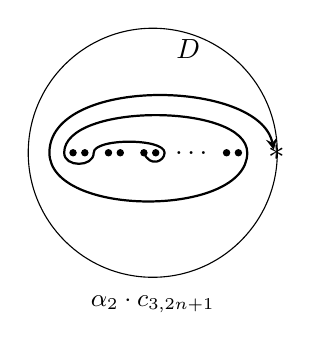
\begin{tikzpicture}[scale=.75,>=stealth]
        % background
        \foreach \c in {5} \draw (\c,1) circle (60pt);
        \foreach \c in {5}
          \foreach \p in {-1.35,-1.15,-.75,-.55,-.15,.05,1.25,1.45} \filldraw (\c+\p,1) circle (1.5pt);
        \foreach \c in {5}  
          \draw   (\c+2.1,1) node {{\large $\ast$}}
              (\c+0.6,2.75) node {$D$};
              %(\c-1,1) node[below] {{\small $i$}}
              %(\c+1,1) node[below] {{\small $j$}};
        \foreach \c in {5}
          \draw (\c+0.65,1) node {$\ldots$};
        %\filldraw  (5,1) circle (1.5pt);
        %\draw  (5,1) node[below] {{\small $k$}};
        % on right
        %\draw[->,thick] (9,1.1) ..controls (9,1.4) and (10.7,2.2) .. (11.685,1.01);
        %\draw (10,-0.75) node[below] {{\small $\sg_{i,j}\cdot c_{j,n+1}$}};
        % on left
        %\draw[->,thick] (1,1.125) ..controls (0.75,1.625) and (-0.25,1.4) ..(-0.75,0.9)
        %             ..controls (-1.1,0.69) and (-1.45,0.99) ..(-1.1,1.2)
        %             ..controls (-0.75,1.41) and (0.7,2.2) ..(1.685,1.01);
        %\draw (0,-0.75) node[below] {{\small $\sg_{i,j}\cdot c_{i,n+1}$}}; 
        % in center
        \draw[->,thick] (4.85,1)  ..controls (4.95,.75) and (5.2,.85) ..(5.2,1)
                      ..controls (5.2,1.25) and (4,1.25) ..(4,1)
                      ..controls (4,.75) and (3.5,.75) .. (3.5,1)
                      ..controls (3.5,1.85) and (6.6,1.85) .. (6.6,1)
                      ..controls (6.6,-.1) and (3.25,-.1) ..(3.25,1)
                      ..controls (3.25,2.3) and (6.8,2.25) ..(7.05,1.05);
        %           ..controls (6.1,0.69) and (6.45,0.99) ..(6.1,1.2)
        %           ..controls (5.2,1.75) and (4.95,1.32) ..(5-0.75,0.9)
        %           ..controls (5-1.1,0.69) and (5-1.45,0.99) ..(5-1.1,1.2)
        %           ..controls (5-0.4,1.62) and (5.7,2.2) ..(6.685,1.01);
        \draw (5,-1.25) node[below] {{\small $\alpha_2\cdot c_{3,2n+1}$}};
      \end{tikzpicture}
      \caption{Computing third row of $\Phi_{\alpha_2}^L$}
      \label{FigPhiLCalcPhi}
    \end{figure}

  Denote the curve on the left in Figure \ref{FigSentToZero} by $x_i$. Denote by $y_{ij}$ the curve on the right in the same figure, and let $y_{ij}=1$ if $i=j$. Using the relation \ref{FigRelnPathAlg} to pull the curve in Figure \ref{FigPhiLCalcPhi} across the rightmost $2n-6$ punctures, we consider how to get a coefficient of $a_{j,2n+1}$. For each $j\ge 7$ we get a coefficient of $a_{j,2n+1}$ as below.

      \begin{equation}\langle\phi_{\alpha_2}^{\ast}(a_{3,2n+1}), a_{j,2n+1}\rangle = \sum_{i=j}^{2n}x_{i}y_{i,j}
      \label{eqnCurveExpansion}
      \end{equation}
    
    \begin{figure}[ht]
      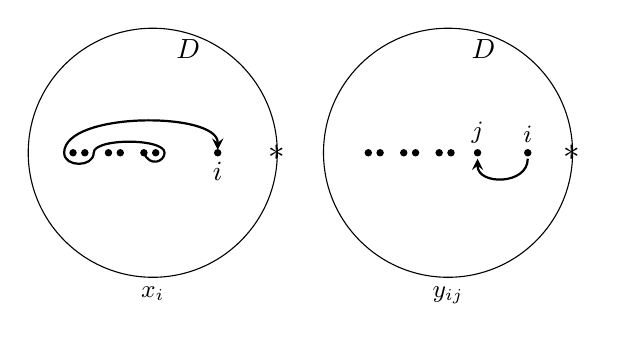
\begin{tikzpicture}[scale=.75,>=stealth]
        % background
        \foreach \c in {2,7} \draw (\c,1) circle (60pt);
          \foreach \p in {-1.35,-1.15,-.75,-.55,-.15,.05,1.1} \filldraw (2+\p,1) circle (1.5pt);
          \foreach \p in {-1.35,-1.15,-.75,-.55,-.15,.05,.5,1.35} \filldraw (7+\p,1) circle (1.5pt);
        \draw (2+1.1,1) node[below] {$i$};
        \foreach \c in {2,7}  
          \draw   (\c+2.1,1) node {{\large $\ast$}}
              (\c+0.6,2.75) node {$D$};
              %(\c-1,1) node[below] {{\small $i$}}
              %(\c+1,1) node[below] {{\small $j$}};
        
        %\filldraw  (5,1) circle (1.5pt);
        %\draw  (5,1) node[below] {{\small $k$}};
        % on right
        %\draw[->,thick] (9,1.1) ..controls (9,1.4) and (10.7,2.2) .. (11.685,1.01);
        %\draw (10,-0.75) node[below] {{\small $\sg_{i,j}\cdot c_{j,n+1}$}};
        % on left
        %\draw[->,thick] (1,1.125) ..controls (0.75,1.625) and (-0.25,1.4) ..(-0.75,0.9)
        %             ..controls (-1.1,0.69) and (-1.45,0.99) ..(-1.1,1.2)
        %             ..controls (-0.75,1.41) and (0.7,2.2) ..(1.685,1.01);
        %\draw (0,-0.75) node[below] {{\small $\sg_{i,j}\cdot c_{i,n+1}$}}; 
        % in center
        \draw[->,thick] (1.85,1)  ..controls (1.95,.75) and (2.2,.85) ..(2.2,1)
                      ..controls (2.2,1.25) and (1,1.25) ..(1,1)
                      ..controls (1,.75) and (.5,.75) .. (.5,1)
                      ..controls (.5,1.7) and (3.1,1.7) .. (3.1,1.05);
        
        \draw[->,thick] (8.35,.9) ..controls (8.35,.45) and (7.5,.45) .. (7.5,.9);
        \draw (7.5,1) node[above] {\small $j$}
              (8.35,1) node[above] {\small $i$};

        \draw (2,1-2.1) node[below] {\small $x_i$}
              (7,1-2.1) node[below] {\small $y_{ij}$};
      \end{tikzpicture}
      \caption{Coefficients that are sent to zero.}
      \label{FigSentToZero}
    \end{figure}

  
  As $x_{2n}$ is the coefficient of $a_{2n,2n+1}$, our assumption makes $\varphi(x_{2n}) = 0$. This in turn implies that $\varphi(x_{2n-1})=0$ by considering the case $j=2n-1$. Continuing in this way, we see that $\varphi(x_{j})=0$ for all $j>6$. Letting $w$ denote the curve of Figure \ref{FigPhiLCalcPhiReduced}, we see that (applying $\varphi$ to the coefficients of the $a_{j,2n+1}$) $\varphi(\phi_{\alpha_2}^{\ast}(a_{3,2n+1})) = \varphi(w)$. We remark, the curve $w$ is the image of $c_{3,2n+1}$ under the braid $\phi_{(\s_1\s_2)_2^4}$ in $B_6\subset B_{2n}$.

    \begin{figure}[ht]
      \begin{tikzpicture}[scale=.75,>=stealth]
        % background
        \foreach \c in {5} \draw (\c,1) circle (60pt);
        \foreach \c in {5}
          \foreach \p in {-1.35,-1.15,-.75,-.55,-.15,.05,1.25,1.55} \filldraw (\c+\p,1) circle (1.5pt);
        \foreach \c in {5}  
          \draw   (\c+2.1,1) node {{\large $\ast$}}
                  (\c+.85,1) node {\small $\ldots$}
                  (\c+0.6,2.75) node {$D$};
              %(\c-1,1) node[below] {{\small $i$}}
              %(\c+1,1) node[below] {{\small $j$}};
        \foreach \c in {5}
        %\filldraw  (5,1) circle (1.5pt);
        %\draw  (5,1) node[below] {{\small $k$}};
        % on right
        %\draw[->,thick] (9,1.1) ..controls (9,1.4) and (10.7,2.2) .. (11.685,1.01);
        %\draw (10,-0.75) node[below] {{\small $\sg_{i,j}\cdot c_{j,n+1}$}};
        % on left
        %\draw[->,thick] (1,1.125) ..controls (0.75,1.625) and (-0.25,1.4) ..(-0.75,0.9)
        %             ..controls (-1.1,0.69) and (-1.45,0.99) ..(-1.1,1.2)
        %             ..controls (-0.75,1.41) and (0.7,2.2) ..(1.685,1.01);
        %\draw (0,-0.75) node[below] {{\small $\sg_{i,j}\cdot c_{i,n+1}$}}; 
        % in center
        \draw[->,thick] (4.85,1)  ..controls (4.95,.75) and (5.2,.85) ..(5.2,1)
                      ..controls (5.2,1.25) and (4,1.25) ..(4,1)
                      ..controls (4,.75) and (3.5,.75) .. (3.5,1)
                      ..controls (3.5,1.5) and (5.5,1.5) .. (5.5,1)
                      ..controls (5.5,.25) and (3.25,.25) ..(3.25,1)
                      ..controls (3.25,2.3) and (6.8,2.25) ..(7.05,1.05);
        %           ..controls (6.1,0.69) and (6.45,0.99) ..(6.1,1.2)
        %           ..controls (5.2,1.75) and (4.95,1.32) ..(5-0.75,0.9)
        %           ..controls (5-1.1,0.69) and (5-1.45,0.99) ..(5-1.1,1.2)
        %           ..controls (5-0.4,1.62) and (5.7,2.2) ..(6.685,1.01);
        \draw (5,-1.25) node[below] {{\small $w = (\s_1\s_2)_2^4\cdot c_{3,2n+1}$}};
      \end{tikzpicture}
      \caption{Reduction of computation}
      \label{FigPhiLCalcPhiReduced}
    \end{figure}
  %(For $i=1,j=1$ is the part of $\phi_{\pp2\tau}^{-1}({\bf a}))$ corresponding to terms in $B_{11}^{n+1}$ really just $a_{ij}\mapsto a_{i+2,j+2}$? {--} note this is what happens with $n=3$.)

  A similar argument to the above shows that the (coefficients of the) image under $\varphi$ of $\alpha_2\cdot c_{4,2n+1}$, $\alpha_2\cdot c_{5,2n+1}$, and $\alpha_2\cdot c_{6,2n+1}$ also correspond to the image of $(\s_1\s_2)_2^4\cdot c_{i,7}$. This implies that $\varphi$, when applied to the $6\times 6$ matrix $\Phi_{(\s_1\s_2)_2^4}^L$, sends the last four rows to ${\bf e}_3,{\bf e}_4,{\bf e}_5,{\bf e}_6$. It can be directly calculated that any such map on $\mathcal A_6$ satisfies $\varphi(-a_{32}) = 0$, concluding the proof of the lemma.
  \end{proof}

To complete the theorem, recall that $K=\hat{\alpha_2\s_1}$. Any augmentation with rank $2n$ would require a homomorphism $\epsilon: \mathcal A_{2n}\to\mathbb C$ such that $\epsilon\left(\Phi_{\alpha_2\s_1}^L\right) = \Delta(\alpha_2\s_1)$. By the Chain rule $\Phi_{\alpha_2\s_1}^L = \phi_{\alpha_2}(\Phi_{\s_1}^L)\Phi_{\alpha_2}^L$ which, by the form of $\Phi_{\s_1}^L$, has (except for the first two rows) the same rows as $\Phi_{\alpha_2}^L$.

As a consequence, $\epsilon$ must send the $i^{th}$ row of $\Phi_{\alpha_2}^L$ to ${\bf e_i}$ for $i\ge 3$. By Lemma \ref{LemZeroness} we see that $\epsilon\left((\Phi_{\alpha_2}^L)_{12}\right) = 0$. As $\Phi_{\alpha_2\s_1}^L = \phi_{\alpha_2}(\Phi_{\s_1}^L)\Phi_{\alpha_2}^L$ indicates that $\Phi_{\alpha_2\s_1}^L$ has a second row equal to the first row of $\Phi_{\alpha_2}^L$, there is a diagonal entry in $\epsilon\left(\Phi_{\alpha_2\s_1}^L\right)$ equal to zero, so it cannot equal $\Delta(\alpha_2\s_1)$, a contradiction.
\end{proof}

\subsection{Augmentation rank does not multiply}
\label{SecMultiplic}

As discussed in Section \ref{SecAsSatelliteOp} the braid satellite $K(\alpha,\beta)$ depends only on $\beta$ and the closure $\hat{\alpha}$ if $\alpha$ has minimal braid index. We give some motivation for Conjecture \ref{ConjSuperMultipl}, that $\ar(K(\alpha,\beta))\ge \ar(\hat{\alpha})\ar(\hat{\beta})$.

\begin{thm}For any braid $\alpha$ with $K=\hat{\alpha}$, we have $\ar(K(\alpha,\beta)) \ge \ar(K)$.
\label{ThmCompanionRank}
\end{thm}
\begin{proof}The knot group $\pi_{K(\alpha,\beta)}$ is isomorphic to a product of $\pi_K$ and the group for the closure of $\Delta^{2\omega}\beta$ amalgamated along a $\mathbb Z^2$ coming from the torus boundary $T$ of the neighborhood $n(K)$. Choose the basepoint of $\pi_{K(\alpha,\beta)}$ on $T$ and include $\pi_K$ into the amalgamated product via the inclusion of the complement.

Let $m_1$ be the meridian of $K$ determined by a based loop contained in $T$ that is contractible in $n(K)$. Suppose that $\rho:\pi_K\to\text{GL}_n\mathbb C$ is an irreducible KCH representation with $\widetilde M = \rho(m_1) = \text{diag}[\widetilde\mu_0,1,\ldots,1]$ for some $\widetilde\mu_0\in\mathbb C\setminus\{0\}$. Choose any $p^{th}$ root $\mu_0$ of $\widetilde\mu_0$. 

Consider a collection of meridians $m_1,\ldots,m_r$ of $K$ that generate $\pi_K$. For each $1\le i\le r$ there are $p$ meridians $m_{i1},\ldots,m_{ip}$ of $K(\alpha,\beta)$ such that $m_{i1}m_{i2}\ldots m_{ip} = m_i$. Set $\s(m_{1j}) = \text{diag}[\mu_0,1,\ldots,1] = M$ for $1\le j\le p$. Then, for each $2\le i\le r$ find $w_i\in\pi_K$ so that $m_i = w_im_1w_i^{-1}$ and set $\s(m_{ij}) = \rho(w_i)M\rho(w_i)^{-1}$ for $1\le j\le p$.

As $\pi_{K(\alpha,\beta)}$ has a presentation with every relation of the form $m_{i,j} = w_im_{1,k}w_i^{-1}$ for some $1\le j, k\le p$ and $1\le i\le r$ we see that $\s:\pi_{K(\alpha,\beta)}\to\text{GL}_n\mathbb C$ is a well-defined KCH representation. Moreover, $\s$ has the same image as $\rho$, implying it is irreducible. This shows that $\ar(K(\alpha,\beta))\ge \ar(K)$.
\end{proof}

It should also be noted that, for $P=\hat{\Delta^{2\omega}\beta}$, we have $\ar(K(\alpha,\beta))\ge \ar(P)$ also. This follows from Proposition \ref{PropAsSatelliteOp} and the fact that there is a surjection $\pi_{K(\alpha,\beta)}\to\pi_P$, preserving peripheral structures (see Proposition 3.4 in \cite{SW}, for example). 

Oddly, the product $\ar(K)\ar(P)$ does not relate well to $\ar(K(\alpha,\beta))$, even when $\alpha$ has minimal index: from Theorem \ref{ThmNNPlus1} we find examples where $\ar(K(\alpha,\beta))<\ar(K)\ar(P)$ and from Theorem \ref{main} there are examples with $\ar(K(\alpha,\beta))>\ar(K)\ar(P)$. However, to our knowledge Conjecture \ref{ConjSuperMultipl} may hold as stated. 

There are cases where $\ar(K(\alpha,\beta))$ is strictly larger than $\ar(K)\ar(\hat{\beta})$. One example can be found from the $(2,11)$-cable of the $(2,5)$ torus knot. By finding a solution to (\ref{eqn:FindingAugs}) for $\alpha = {\scriptstyle \bar{\bar{2}}}\s_1^5\cdot \s_1\in B_4$, we can compute that $\ar(K(\s_1^5,\s_1)) = 4$, even though $\ar(\hat{\s_1^5})=2$ and $\ar(\hat{\s_1})=1$. Unfortunately, any more examples of cables of torus knots (not covered by Theorems \ref{main} and \ref{ThmNNPlus1}) seem outside of our computational abilities.

We end with a simple remark on computational observations. By the inequalities in (\ref{cor:DimBound}) if a knot has bridge number less than its minimal braid index $n$, it cannot have augmentation rank equal to $n$. Take a minimal index braid representative of such a knot, and multiply that braid by successively higher powers of $\Delta^2\in B_n$, testing in each instance if the closure has augmentation rank equal to $n$. In examples, the power of $\Delta^2$ need not be very high, compared to $n$, before a braid with augmentation rank $n$ appears. The existence of such an augmentation also seems to persist. Note that braids which are sufficiently far in Dehornoy's order from the identity were shown in \cite{MN} to not admit a Birman-Menasco template, and thus are minimal index representatives by the MTWS. For a given braid index $n$, is there a number $m_n$ such that whenever $\Delta^{2m_n}$ is less than $\alpha\in B_n$ in the Dehornoy order, then $\ar(\hat{\alpha}) = n$?

\bibliography{AugsCables_refs}
\bibliographystyle{alpha}
\end{document}
